\documentclass[a4paper, 12pt]{report}
\usepackage[utf8x]{inputenc}
\usepackage[italian]{babel}
%\usepackage[T1]{fontenc}
\usepackage{graphicx}
\usepackage{float}
\usepackage[centertags]{amsmath}
\usepackage{amsfonts}
\usepackage{amssymb}
\usepackage{amsthm}
\usepackage{newlfont}
\usepackage{fancyhdr}
\usepackage{tesisty}
\usepackage{tabularx}
\usepackage{parskip}
\usepackage{comment}


%-------------------------------
% DEFINIZIONE DEGLI ENVIRONMENT
%-------------------------------

%newtheorem{obs}{Osservazione}[section]
%newenvironment{oss}
%   {\begin{obs}\begin{normalfont}}
%   {\hfill $\square \!\!\!\!\checkmark$ \end{normalfont}\end{obs}}

%newtheorem{pro}{Problema}[chapter]
%newenvironment{prob}
%   {\begin{pro}\begin{normalfont}}
%   {\hfill $\spadesuit$ \end{normalfont}\end{pro}}

%newtheorem{teor}{Teorema}[section]
%newenvironment{teorema}
%   {\begin{teor}\textit }
%   {\hfill  \end{teor}}

%newtheorem{defn}{Definizione}[section]
%newenvironment{de}
%   {\begin{defn}\begin{normalfont}}
%   {\hfill $\clubsuit$ \end{normalfont}\end{defn}}

%-----------------------------
% CONFIGURAZIONE DELLA PAGINA
%-----------------------------

\hfuzz2pt % Don't bother to report over-full boxes if over-edge is < 2pt

\fancypagestyle{plain}{
\fancyhead{}\renewcommand{\headrulewidth}{0pt} } \pagestyle{fancy}
\renewcommand{\chaptermark}[1]{\markboth{\small CAP. \thechapter \textit{ #1}} {} }
\renewcommand{\sectionmark}[1]{\markright{\small  \thesection \textit{ #1}} {} }
\voffset=-20pt    % distanza tra il limite superiore del foglio e l'intestazione
\headsep=40pt     % distanza  l'intestazione ed il testo del corpo
\hoffset=0 pt     % misura equivalente al margine sinistro
\textheight=620pt % altezza del corpo del testo
\textwidth=435pt  % larghezza del corpo del testo
\footskip=40pt    % distanza tra il testo del corpo ed il pie' di pagina
\fancyhead{}      % cancella qualsiasi impostazione per l'intestazione
\fancyfoot{}      % cancella qualsiasi impostazione per il pie' di pagina
\headwidth=435pt  % larghezza del'intestazione e del pie' di pagina
\fancyhead[R]{\rightmark} \fancyfoot[L]{\leftmark}
\fancyfoot[R]{\thepage}
\renewcommand{\headrulewidth}{0.3pt}   % spessore della linea dell'intestazione
\renewcommand{\footrulewidth}{0.3pt}   % spessore della linea del pi�di pagina

\numberwithin{equation}{section}
\renewcommand{\theequation}{\thesection.\arabic{equation}}


\begin{document}


\dedicate{Ai miei nonni.}

\corso{INGEGNERIA INFORMATICA} \titoloTesi{CASO DI STUDIO ED APPLICAZIONE DI UNA SOLUZIONE DEVOPS IN AMBIENTE ENTERPRISE} \ciclo{Ciclo}
\anno{2018-2019}
\relatore{Prof. Maurizio Patrignani}
\autore{Leonardo Albanese}
\correlatore{Ing. Alessandro Casula}
\baselineskip=25pt
\intestazione
%------------------------------------------------
% INTRODUZIONE E RINGRAZIAMENTI (NON MODIFICARE)
%------------------------------------------------

\fancypagestyle{plain}{
\fancyhead{}\renewcommand{\headrulewidth}{0pt} } \pagestyle{fancy}
\renewcommand{\chaptermark}[1]{\markboth{\small Cap. \thechapter \textit{ #1}} {} }
\renewcommand{\sectionmark}[1]{\markright{\small  \S \thesection \textit{ #1}} {} }
\voffset=-20pt                         % distanza tra il limite superiore del foglio e l'intestazione
\headsep=40pt                          % distanza  l'intestazione ed il testo del corpo
\hoffset=0pt                           % misura equivalente al margine sinistro (orig 0pt)
\textheight=620pt                      % altezza del corpo del testo
\textwidth=435pt                       % larghezza del corpo del testo (orig 435pt)
\footskip=40pt                         % distanza tra il testo del corpo ed il pie' di pagina
\fancyhead{}                           % cancella qualsiasi impostazione per l'intestazione
\fancyfoot{}                           % cancella qualsiasi impostazione per il pie' di pagina
\headwidth=435pt                       % larghezza del'intestazione e del pie' di pagina
\fancyhead[R]{\rightmark} \fancyfoot[L]{\leftmark}
\fancyfoot[R]{\thepage}
\renewcommand{\headrulewidth}{0.3pt}   % spessore della linea dell'intestazione
\renewcommand{\footrulewidth}{0.3pt}   % spessore della linea del pi�di pagina

\pagenumbering{Roman} \tableofcontents
\newpage

\pagenumbering{arabic}

\fancyhf{} %elimina header/footer vecchi

\fancyhead[R]{Introduzione}\fancyfoot[L]{Introduzione}
\fancyfoot[R]{\thepage}

\include{Introduzione}

\chapter*{Introduzione}
\addcontentsline{toc}{chapter}{Introduzione}

Questa tesi, svolta all'interno di una grande azienda di telecomunicazioni, si propone come obiettivo l'illustrazione di una possibile implementazione di una piattaforma per l'applicazione della metodologia DevOps in un ambiente enterprise internazionale di elevata complessità. La necessità di conciliare processi blindati e consolidati da anni con i nuovi ritmi dettati dalla competizione sempre più accesa permettono di evidenziare i benefici che una simile soluzione possa portare all'interno di contesti simili.\\
Questo documento espone i requisiti che un'organizzazione aziendale deve avere per poter applicare correttamente questo tipo di tecnologia, i processi decisionali che hanno portato alla definizione dell'infrastruttura di supporto ed all'utilizzo dei software e delle tecnologie necessarie ed infine la dimostrazione pratica del funzionamento dell'infrastruttura, correlata da alcuni esempi tecnici e diagrammi di sequenza.\\
Nel capitolo \ref{motivazioni} sono descritte le ragioni per cui la competitività del mercato e l'introduzione di nuovi trend tecnologici abbiano portato alla necessità di uno svecchiamento dei vecchi processi, che tuttavia non possono essere completamente dismessi in funzione delle nuove metodologie, ma che vanno invece modificati ed integrati dove possibile, dando vita ad una soluzione unica per l'azienda che la vuole utilizzare, ma anche ad un modello per altre aziende che vivono un simile contesto.\\
Nel capitolo \ref{metodologie} sono elencate le metodologie che vengono studiate ed applicate per il design dell'infrastruttura e per la scelta dei software da utilizzare, assieme ad un confronto con i processi attuali. Per ogni metodologia è fornita una descrizione generale con i riferimenti alla letteratura per un eventuale approfondimento.\\
Nel capitolo \ref{tecnologie} sono elencate le tecnologie alla base dei software che compongono l'infrastruttura, con una descrizione generale del loro funzionamento e riferimenti alla documentazione per un eventuale approfondimento.\\
Nel capitolo \ref{requisiti} viene fornita una visione generale delle attuali organizzazioni aziendali, in contrasto con le nuove tecnologie. Quindi viene fornito un esempio di nuova organizzazione in linea con i principi dell'Agile, assieme ai requisiti di natura funzionale e tecnica che la soluzione caso di studio deve soddisfare.\\
Nel capitolo \ref{teams} sono elencati i team che prendono parte nel processo della soluzione DevOps, confrontando l'evoluzione che hanno i loro compiti dal processo attuale all'utilizzo delle nuove metodologie.\\
Nel capitolo \ref{software} è descritto il processo decisionale che porta alla scelta dei software per ogni componente dell'infrastruttura, assieme ad uno studio sulla scelta tra strumenti open source e proprietari.\\
Nel capitolo \ref{concetti-devops} vengono descritte le componenti tecniche, in termini di workflow e componenti, che vengono utilizzate per integrare al loro interno qualsiasi tipologia di sviluppo software, da applicazioni monolitiche a quelle a microservizi.
Nel capitolo \ref{tech} sono approfonditi due dei processi inclusi all'interno della piattaforma, quelli nei quali ho preso parte attivamente, correlati da diagrammi di sequenza, che mostrano le comunicazioni infrastrutturali tra i componenti che fanno parte della piattaforma DevOps, relativamente ad un'applicazione a microservizi.\\
Nel capitolo \ref{piattaforma-devops} sono mostrati i flussi integrati all'interno della soluzione DevOps, che comprendono tutte le tipologie di aggiornamenti software, in modo da mostrare come tale tecnologia possa essere indipendente dalle tecnologie utilizzate.\\
Nel capitolo \ref{conclusioni} sono tratte le conclusioni e osservati dove possibili i benefici della soluzione implementata, in termini di prima e dopo.\\
Questo documento, dovendo osservare i limiti imposti dalla politica della divulgazione di materiale aziendale, non intende essere un manuale applicativo, perciò alcuni aspetti tecnici sono volutamente descritti in maniera superficiale.
\newpage



\fancyhf{} %elimina header/footer vecchi


\fancyhead[R]{\rightmark} \fancyhead[L]{\leftmark}
\fancyfoot[R]{\thepage}





%---------------------
% INCLUSIONE CAPITOLI
%---------------------

\chapter{Motivazioni}\label{motivazioni}
Il tema dell’Agile e di tutto ciò che è di contorno, compresa la filosofia DevOps, nonostante abbia cominciato a svilupparsi agli inizi del 2000, è ancora un argomento di discussione, studio e metodologie di applicazione. Per la sua effettiva capacità di portare maggiore efficienza e snellimento dei processi un numero sempre maggiore di organizzazioni vi si avvicina per poter accrescere la propria competitività nel mercato.\\
Le migliori applicatrici delle pratiche Agile e DevOps sono le startup, piccole aziende, normalmente nate negli ultimi 5-10 anni, con un numero ristretto di dipendenti, solitamente giovani e che quindi hanno iniziato a sviluppare prodotti già secondo queste metodologie e perciò non influenzati da bad practice pregresse.\\
In queste nuove realtà, dove il contesto di applicazione della DevOps è una tabula rasa su cui poter lavorare in completa libertà, si tende a seguire pedissequamente la letteratura, ma questo approccio non è applicabile ad organizzazioni strutturalmente molto più complesse di dimensioni spesso internazionali, perché vi sono restrizioni dettate dall’organizzazione aziendale, dalla difficoltà di aprirsi al cambiamento e dalla presenza di processi interni dell’azienda che spesso si trovano in contrasto con le pratiche Agile.
Lo scopo di questo caso di studio è quello di esporre una proposta di applicazione di una piattaforma DevOps in un’enterprise multinazionale che per necessità organizzative e legali necessita di mantenere un certo standard di sicurezza e controllo sui processi, ma che allo stesso tempo ha l'esigenza di adeguarsi all’aumentata competitività del mercato, riducendo il time to market e i costi per poter rispondere velocemente ai nuovi trend introdotti dalla concorrenza.\\
Poiché le metodologie DevOps mostrano offrono maggiore potenzialità soprattutto nello sviluppo di 
applicazioni a microservizi, la tesi utilizza tale applicazione come esempio per la messa
in pratica e la verifica di correttezza del processo, mostrando perciò i legami che
intercorrono tra un'applicazione con tale struttura e le metodologie Agile.


\chapter{Metodologie applicate}\label{metodologie}
In questo capitolo vengono elencate le tecnologie utilizzate per la realizzazione dell’infrastruttura e l’organizzazione dei task. 
\section{Metodologia Agile}\label{agile}
Questo paragrafo intende esporre la metodologia Agile nei suoi aspetti ed obiettivi principali, per approfondimenti sull’argomento si rimanda alla consultazione degli articoli citati a piè di pagina.\\
La metodologia Agile racchiude un elenco di principi e filosofie dell’ingegneria del software che possono essere riassunti in quattro punti fondamentali, descritti nel manifesto Agile \cite{manifesto-agile}, che sottolineano la maggiore importanza di:
\begin{enumerate}
    \item Gli individui e le interazioni, più che i processi e gli strumenti
    \item Il software funzionante, più che la documentazione esaustiva
    \item La collaborazione col cliente, più che la negoziazione dei contratti
    \item Rispondere al cambiamento, più che seguire un piano
\end{enumerate}
Cominciata a svilupparsi all’inizio degli anni 2000, oggi è una best practice affermata ed utilizzata da un numero sempre crescente di aziende per via della sua effettiva capacità di portare beneficio ai membri del team e alle organizzazioni stesse. \\
Nel tradizionale approccio a cascata la consultazione con il cliente avviene solamente durante la fase di definizione dei requisiti e alla presentazione del prodotto finito, passando attraverso fasi di design, coding, testing che vengono eseguite in maniera sequenziale, una dietro l’altra \cite{palmquist-agile}, accompagnate da un'elevata mole di documentazione. Questa visione del progresso espone l’intero processo a delle vulnerabilità basate sul concetto che i requisiti per un software possono variare nel tempo e questi cambiamenti dovrebbero poter essere facilmente integrati nel software. Su questa vulnerabilità del metodo “tradizionale”, l’approccio Agile fonda il suo  punto di forza.\\ 
La parola “agile”, di trascrizione italiana, ma pronuncia inglese, sta ad indicare la capacità di adattarsi al cambiamento caratteristica dei team e delle organizzazioni che adottano questa filosofia \cite{balaji-agile}. Questa capacità viene acquisita passando dal macrociclo dell’approccio a cascata ad una sequenza di cicli di dimensioni minori, più facilmente controllabili e gestibili, in grado di fornire un continuo feedback sul lavoro svolto, sia da parte del team, che da parte del cliente stesso, così che miglioramenti del codice o cambiamenti nei requisiti possano essere tempestivamente integrati all’interno dello sviluppo. \\
Mentre alcune filosofie facenti parte della metodologia Agile come Extreme Programming e Feature Driven Development pongono la propria attenzione sul prodotto, altre come Scrum e Kanban \cite{kumar-agile}  pongono il focus sul team, in modo da massimizzare la produttività e diminuire lo stress degli sviluppatori \cite{melo-agile}.\\
All’interno di questo progetto la metodologia Agile è stata utilizzata come linea guida per lo sviluppo e l’implementazione dell’infrastruttura DevOps, la descrizione del rapporto tra questi elementi è presente nei capitoli successivi.
\subsection{Applicazione di Scrum e Kanban per l'Agile}
Kniberg mostra che un utilizzo coordinato di Scrum e Kanban, porta una maggiore efficienza nell'organizzazione del lavoro del team, rendendola più Agile \cite{kniberg-agile}.\\
%Scrum e Kanban sono due approcci della filosofia Agile che possono essere utilizzati in maniera coordinata per ottenere un’organizzazione del lavoro più “agile” \cite{kniberg-agile}.
Scrum è un framework per la gestione del ciclo di sviluppo software che consiste in passi incrementali in cui ogni fase del progresso è sottoposta a feedback e migliorie tramite una comunicazione garantita da stand-up meeting quotidiani, spring review ogni due settimane e backlog. Questa gestione dello sviluppo si rispecchia anche nell’organizzazione dei team, che sono ridimensionati e focalizzati su task più compatti e più semplici da gestire \cite{schwaber-agile}.\\
Kanban è una metodologia di sviluppo software basato sul sistema ideato dal Toyota Production System che si propone di gestire il flusso di lavoro in maniera efficace tramite la riduzione del Work in Progress e un costante monitoraggio del workflow per migliorarlo e renderlo più efficiente \cite{klipp-agile}.\\
All’interno del progetto, sono state utilizzate entrambe le metodologie, per ottenere un risultato in linea con la filosofia agile.\\
All’inizio di ogni giornata si partecipa ad uno “Stand-up meeting”, della durata variabile tra 15 e 20 minuti \cite{hasnain-agile}, dove ogni membro del team espone il lavoro svolto fino a quel momento, gli obiettivi del giorno e se ha riscontrato qualche difficoltà bloccante nello sviluppo. Nel caso vi fossero difficoltà di comprensione del lavoro svolto, o necessità di condividere delle conoscenze per poter continuare lo sviluppo, queste vengono risolte attraverso un confronto in sede differente (per non allungare la durata del meeting).\\
A seguito di questo incontro, la Kanban board, una board che mostra quattro colonne: “To Do”, “In progress”, "Pending"\footnote{La presenza del campo "Pending", che non trova spazio in letteratura, è stata introdotta per quei task che risultano in attesa dell'azione di un ente esterno.} e “Done”, viene aggiornata inserendo i task spettanti a ciascun membro del team, così da avere sempre sotto controllo il workflow dello sviluppo e per suddividere le responsabilità in modo da non sovrapporre i flussi di lavoro.\\


\section{DevOps}\label{devops}
I rilasci del software in ambiente di produzione rappresentano la parte più critica per il business di un’azienda: un rilascio di codice affetto da bug, effettuato in ritardo o che porta il sistema in uno stato inconsistente può tradursi per l’organizzazione in un danno economico e d’immagine non indifferenti \cite{garfinkel-agile}. Allo stesso tempo, un programma, finché non viene rilasciato, non porta alcun vantaggio di business.\\
L’adozione della metodologia DevOps contribuisce a diminuire il rischio legato ai rilasci con i seguenti benefici \cite{wikipedia-devops-agile}:
\begin{itemize}
    \item \emph{Minore costo delle modifiche}: l'adozione del modello agile o modello incrementale, in contrasto con il tradizionale modello a cascata, comporta modifiche meno costose, anche se più frequenti, con minore impatto e rischio.
    \item \emph{Maggiore coordinamento dei rilasci}: la presenza di una coordinazione del rilascio riduce le distanze tra sviluppo e gestione.
    \item \emph{Automazione}: una completa automazione assicura la facile ripetibilità dei rilasci e riduce gli errori nel processo.
\end{itemize}
Il termine \emph{DevOps} deriva dalla contrazione dei due termini inglesi “Development” e “Operations” che corrispondono alle fasi dello sviluppo e del rilascio in produzione del software. Poiché queste due rappresentano gli estremi della catena di produzione del software, la DevOps mira ad incentivare la comunicazione e collaborazione tra sviluppatori e gli addetti alle operations per ottenere un prodotto di migliore qualità e con un minore time to market \cite{hutterman-iac}.\\
Uno dei maggiori vantaggi nell’adozione di un approccio di questo tipo è l’abilitazione della Continuous Delivery \cite{chen-devops}, ovvero il rilascio continuo di software attraverso una sequenza di step sottoposti a feedback continui per sottoporre il processo stesso ad un miglioramento continuo e per garantire la miglior qualità possibile dei rilasci.\\
Relativamente allo sviluppo di architetture a microservizi, dove il rilascio di nuove funzionalità del software possono avvenire in maniera indipendente tra un componente e l’altro, la DevOps e la CD trovano la loro applicazione più naturale \cite{balalaie-devops}.
La pratica della DevOps trova le fondamenta della sua esistenza nella metodologia Agile, tanto che la mancanza della seconda non potrebbe portare ad una corretta adozione della prima \cite{lwakatare-devops}, in quanto la necessità di adattarsi ai cambiamenti è favorita dalla possibilità di poter effettuare rilasci frequenti, automatici e ripetibili.

\section{Continuous Delivery/Deployment/Integration}
Nell'approccio tradizionale il rilascio del software consiste nell’esecuzione di una sequenza di istruzioni, descritte in una dettagliata documentazione, attraverso comandi impartiti da interfaccia testuale. Questo approccio, oltre a causare nell’addetto alle Operations una sensazione di “incubo” del rilascio, introduce un’elevata probabilità d’errore umano. \\
Dalla necessità di snellire il processo di rilascio del software e l’esigenza di processi automatici per la gestione di programmi sempre più complessi e composti da componenti indipendenti tra loro, trova applicazione la Continuous Delivery.\\ 
La Continuous Delivery (CD) è un approccio dell’ingegneria del software dove i team producono software in cicli brevi, assicurando così che il software possa essere teoricamente rilasciato in qualsiasi momento manualmente \cite{chen-devops}. L’obiettivo cardine è quello di garantire che il software si trovi sempre in uno stato consistente, pronto per essere rilasciato.\\
\begin{figure}
    \centering
    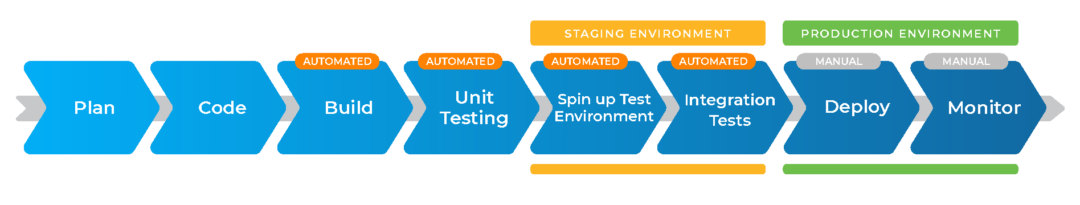
\includegraphics[width=0.9\textwidth]{imgs/cdci.png}
    \caption{Pipeline della Continuous Delivery}
    \label{fig:cd}
\end{figure}
A causa dell'obiettivo comune, spesso, i termini DevOps e Continuous Delivery vengono sovrapposti, ma DevOps è l’insieme di pratiche di organizzazione e di management dei team, rappresentando una “filosofia” da perseguire per lo sviluppo del software, CD è un approccio che mira ad automatizzare il processo per garantire rilasci del software più frequenti e meno soggetti ad errori \cite{humble-devops}. In pratica si potrebbe dire che la DevOps nasce come esigenza nell’applicazione dell’approccio Continuous Delivery in un contesto Agile \cite{lwakatare-devops}.\\
\begin{figure}
    \centering
    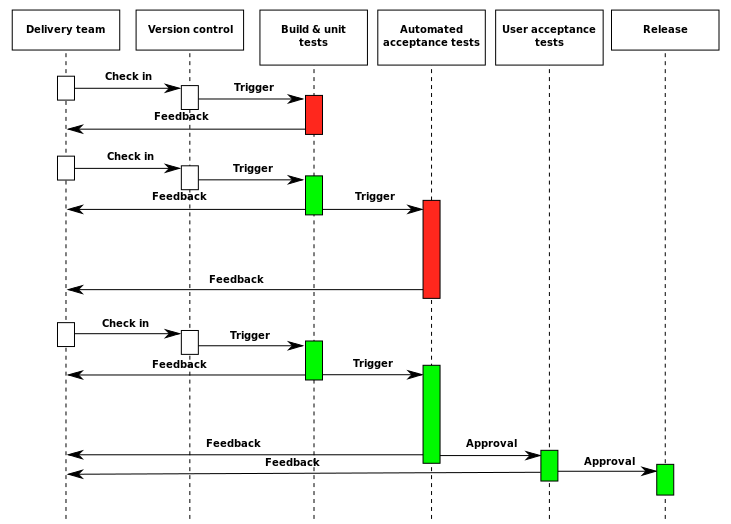
\includegraphics[width=0.9\textwidth]{imgs/cd-funzionale.png}
    \caption{Flusso descrittivo della Continuous Delivery}
    \label{fig:cd-flux}
\end{figure}
Il Continuous Deployment è un concetto simile a quello della Continuous Delivery, ma si differenzia da quest’ultima perché prevede che anche il rilascio in produzione sia oggetto di automatismo.
\begin{figure}[H]
    \centering
    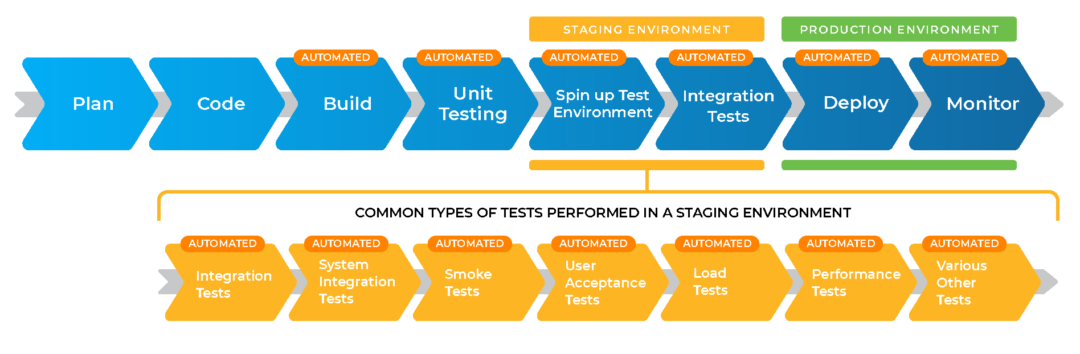
\includegraphics[width=0.9\textwidth]{imgs/continuous-deployment.png}
    \caption{Pipeline del Continuous Deployment}
    \label{fig:my_label}
\end{figure}
La Continuous Integration interviene laddove sia necessario che lo sviluppo del sotware sia sottoposto ad un sistema di controllo di versione. Consiste nell’allineamento frequente dell'ambiente di lavoro degli sviluppatori con l’ambiente condiviso. Questa esigenza nasce dalla problematica legata allo sviluppo di porzioni di codice in maniera indipendente per lunghi periodi di tempo, che potrebbe portare ad errori nel software.\\
Per ottenere un utilizzo corretto della Continuous Integration, Fowler, nel suo famoso articolo del 2006 \cite{fowler-ci}, elenca una lista di requisiti, considerati ormai delle best practice:
\begin{itemize}
    \item Un singolo repository per il codice
    \item Automatizzare il processo di build
    \item La build deve includere test automatici
    \item Ogni sviluppatore deve effettuare dei commit sul repository centrale ogni giorno
    \item Per ogni commit di ogni sviluppatore deve essere eseguita la build di tutto il codice
    \item Intervenire immediatamente sulle build che falliscono
    \item Mantenere veloce il processo di build
    \item Effettuare i test in un ambiente clone di quello di produzione
    \item Ogni sviluppatore deve poter visualizzare il log dell'ultima build
    \item Tutti possono vedere ciò che accade
    \item Rilascio automatico
\end{itemize}
\section{Infrastructure as Code}
L’introduzione di automatismi non riguarda solamente le fasi di build e di rilascio del software, ma anche la definizione di infrastrutture. Le possibilità introdotte dall’uso massiccio del cloud computing permettono la rapida creazione e distruzione di ambienti configurati appositamente secondo le esigenze del software. Gli ambienti, assieme ai componenti che ne fanno parte, hanno bisogno di essere anzitutto correttamente configurati, ma anche riproducibili, cioè si deve essere certi che lo stato di un’infrastruttura possa essere riprodotto su un numero indefinito di istanze di quella infrastruttura.
Ad oggi l'approccio “infrastructure-as-code” comprende tutti quegli automatismi che non riguardano il rilascio del software stesso \cite{hutterman-iac}, quindi legati sia all'infrastruttura che alla configurazione delle macchine che la compongono.\\
Applicativi come Terraform si interfacciano con la piattaforma cloud per configurare le risorse necessarie alla creazione dell’ambiente, altre, come Ansible, Puppet e Chef, si occupano di configurare la macchina eseguendo dei comandi sulle macchine che la compongono.\\
I software di Infrastructure as Code tendenzialmente prevedono la presenza di due tipologie di macchine: nodi e server controllori. I file di configurazione si trovano sulla macchina controllore che poi, tramite un agent, o una connessione SSH (nel caso di Ansible), li eseguono sul nodo garantendo che lo stato della macchina sia sempre quello desiderato.


\chapter{Tecnologie utilizzate}\label{tecnologie}
In questo capitolo sono elencate le tecnologie utilizzate all’interno del progetto. Nei capitoli successivi viene descritto il loro utilizzo più pertinentemente alla piattaforma DevOps.

\section{Tracciatore di issue/bug}
Un tracciatore di issue è un software che ha lo scopo di mantenere uno storico delle segnalazioni degli utenti, bug, nuove iniziative sul software, etc. 
Solitamente è costituito da un database e un’interfaccia via browser che fornisce servizi di ricerca testuale o tramite l’inserimento di query.\\
Con issue si intende una qualsiasi problematica, segnalata dal cliente o dal team di sviluppo stesso. Rappresenta un compito che deve essere preso in carico, gestito e risolto, in un arco di tempo che dipende dalla priorità dell’issue stessa. Ad esempio un bug che non permette di inserire dei nuovi ordini all’interno di una piattaforma di e-commerce deve essere risolto in un tempo molto più stretto rispetto a quello necessario per risolvere la richiesta di un singolo utente che, ad esempio, non riesce a visualizzare la schermata riepilogativa del proprio ordine.\\
Un issue è caratterizzata da una chiave identificativa, una priorità, la persona che ha preso in carico la risoluzione e una sua descrizione; nel caso si tratti di un bug: le circostanze in cui si è verificato e i passaggi per poterlo riprodurre assieme altre informazioni utili per la risoluzione.
Quando un tracciatore di issue viene utilizzato per gestire le iniziative all’interno di un progetto software, senza rapportarsi al cliente, è chiamato tracciatore di bug.

\section{Wiki}
Un progetto software, per poter essere compreso ed utilizzato rapidamente, deve portare con sé un insieme di informazioni che costituiscono la sua documentazione. Questa può essere di due tipi:
\begin{itemize}
    \item \emph{Funzionale}: dove il comportamento e gli obiettivi del software sono descritti ad alto livello, così che il suo funzionamento possa essere facilmente compreso anche da personale non tecnico
    \item \emph{Tecnico}: il funzionamento del software è descritto a basso livello, con riferimento a concetti specifici dell’ingegneria, necessario per facilitare la collaborazione tra i membri del team
\end{itemize}
Questa documentazione deve essere raccolta e catalogata in un software che permetta una facile navigazione, ricerca ed aggiunta di documenti.\\
Un software di wiki è uno strumento di collaborazione che permette a più persone impiegate sul medesimo progetto di scambiarsi informazioni in un filesystem condiviso, da un’interfaccia web acceduta attraverso il browser e dotato di funzioni per il mark up testuale.

\section{Controllo di versione}
Con controllo di versione si intendono tutte quelle azioni che permettono di tenere traccia delle modifiche effettuate a documenti testuali da parte di un gruppo di persone. Nel caso di un progetto software, i documenti testuali sono costituiti dal codice sorgente di cui è composto il programma e le persone sono gli sviluppatori che operano sul progetto stesso.
Il controllo di versione assegna un identificativo numerico ad ogni modifica effettuata e ad essa associa il nome della persona che ha effettuato la modifica.\\
I software che permettono di eseguire il controllo di versione possono operare in due modalità:
\begin{itemize}
    \item \emph{Distribuito}: ogni sviluppatore possiede il proprio repository e lavora su di esso, allineandolo in un secondo momento con il repository remoto
    \item \emph{Centralizzato}: ogni sviluppatore effettua le proprie modifiche direttamente sul repository remoto
\end{itemize}
Oltre a queste due macrodifferenze, solitamente i software di versionamento permettono le stesse funzionalità, ossia la creazione di branch e la gestione dei conflitti (il merge di due modifiche sullo stesso file).

\section{Automazione dello sviluppo}
Per build si intende l’insieme delle attività che permettono di trasformare il codice sorgente in un artefatto che può essere eseguito direttamente dalla macchina. La compilazione del codice è solo una parte del processo, altre attività includono l’analisi statica del codice, il download delle librerie necessarie, l’esecuzione di test automatici.\\
Necessaria per garantire una corretta implementazione della CI è l’automazione di questo processo. Gli strumenti che eseguono questo compito solitamente lavorano utilizzando due approcci \cite{clark-automation}:
\begin{itemize}
    \item \emph{Task-oriented}: le dipendenze vengono soddisfatte eseguendo un set di task imperativi (esempi sono Make, Ant, CMake, etc.)
    \item \emph{Product-oriented}: descrivono le dipendenze rispetto al prodotto che generano (Maven, Gradle, etc.)
\end{itemize}
Alla prima categoria appartengono quegli strumenti che utilizzano un file che contiene un elenco di istruzioni esplicite da eseguire in un certo ordine.\\
Alla seconda categoria appartengono tutti quegli strumenti di build automation che utilizzano un file di properties, solitamente scritto in XML, che descrive le dipendenze del software senza la necessità di dover scrivere esplicitamente le istruzioni da eseguire.
\section{Gitflow workflow}
Gitflow workflow è una best practice di utilizzo di Git per facilitare lo sviluppo concorrente di funzionalità da parte del team di sviluppo.\\
Come esposto da Driessen \cite{driessen-gitflow}, il modello prevede la presenza di due branch principali:
\begin{itemize}
    \item Un branch \textbf{master} che contiene la versione del codice presente in produzione
    \item Un branch \textbf{develop} che contiene lo sviluppo relativo alle nuove funzionalità. Si utilizza come best practice la creazione di un short-lived feature branch che contiene il codice relativo alla nuova funzionalità e richiedere una pull-request prima che il feature-branch sia mergiato su develop. Il team di sviluppo deve garantire che develop sia sempre funzionante e rilasciabile.
\end{itemize}
\begin{figure}
    \centering
    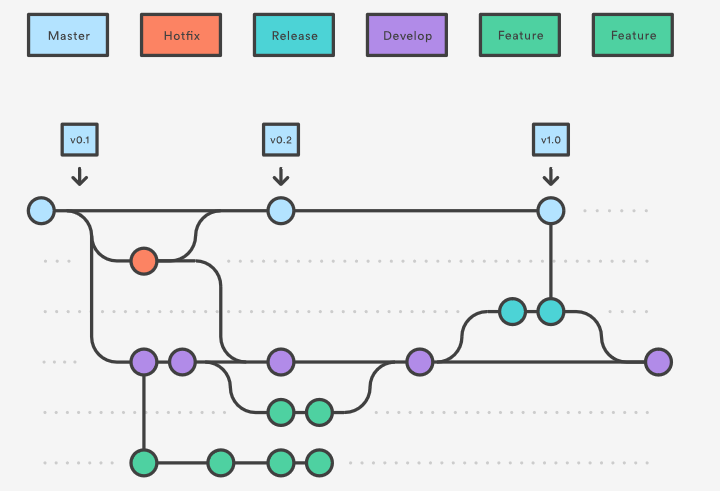
\includegraphics[width=0.9\textwidth]{imgs/gitflow.png}
    \caption{Modello descrittivo del Gitflow \cite{atlassian-doc}}
    \label{fig:gitflow}
\end{figure}
Il programmatore effettua il clone del repository ed il checkout del branch develop. Dopodiché, quando deve integrare una modifica al codice sorgente, dal branch di develop stacca un \textbf{feature} branch, su cui esegue i propri sviluppi ed i commit. Una volta che lo sviluppatore ritiene di aver terminato il suo lavoro, e dopo aver effettuato dei test unitari, il feature branch viene mergiato sul branch di develop.\\
Quando c’è bisogno di rilasciare le nuove modifiche del codice, un branch \textbf{release} viene staccato da develop, su di esso si effettuano dei test, si risolvono bug, si scrive documentazione. Se non vengono rilevati errori, la release una volta rilasciata in produzione viene mergiata sia sul branch master che sul branch develop.\\
Nel caso in produzione siano rilevati dei bug impattanti per il business, che necessitano di una risoluzione immediata, viene staccato dal branch master, che rappresenta la copia del codice attualmente deployato in produzione, un branch \textbf{hotfix} al cui interno si effettuano tutte le modifiche del codice necessarie per risolvere il problema. Quando il bug è risolto ed il codice è stabile, il branch hotfix viene mergiato sia su master che su develop, per mantenerli allineati.\\
All’interno del progetto, la fase di fork e merge dei branch è gestita in maniera automatica tramite delle azioni all’interno del tracciatore di issue, così da permettere allo sviluppatore di concentrarsi solo sulla scrittura del codice.

\section{Microservizi}
Un microservizio è un servizio piccolo e autonomo, eseguito come un processo distinto, che lavora insieme ad altri microservizi comunicando mediante meccanismi leggeri.\\
Per definizione i microservizi sono ottimi candidati all’esecuzione su contenitori, in quanto possono essere gestiti in maniera indipendente, sono autonomi ed espongono le proprie funzionalità tramite un’interfaccia che nasconde agli altri servizi la logica interna.\\
Inoltre i microservizi ben si adattano alla filosofia agile in quanto hanno dimensioni contenute e possono essere gestiti da team di dimensioni ridotte.\\
L’architettura a microservizi si presta per quelle applicazioni dinamiche che hanno bisogno di alta scalabilità, alta disponibilità e un’elevato grado di agilità, cioè che devono saper adattarsi rapidamente alle necessità del business.

\section{Contenitori, Docker e orchestratori di contenitori}\label{containers}
Nel mondo del software, un contenitore è un metodo di virtualizzazione hardware che si differenzia dall’approccio tradizionale per una maggiore leggerezza e versatilità d’uso \cite{felter-containers}. Ogni istanza di contenitore fa riferimento ad un’immagine che comprende le librerie e le dipendenze necessarie per far funzionare l’applicazione rilasciata all’interno del contenitore. Il vantaggio principale di questa tecnologia è la velocità con cui un contenitore può essere creato e distrutto e ciò risulta fondamentale nell’utilizzo enterprise, poiché garantisce la continuità di servizio anche a fronte di guasti o fallimenti.\\
Mentre le macchine virtuali contengono una propria versione completa del sistema operativo, i contenitori utilizzano in maniera condivisa il kernel del sistema operativo della macchina host e lo estendono con le librerie necessarie, questo permette ai contenitori di essere più responsivi alla creazione e alla distruzione e permette un risparmio economico in quanto i contenitori sono di dimensioni contenute e il numero di istanze per host aumenta rispetto alle macchine virtuali tradizionali.
I processi nei contenitori vengono visti dalla macchina host come processi software e l’accesso ad ogni file viene eseguito come l’accesso ad un file nel sistema host, senza l’overhead introdotto da una completa virtualizzazione di sistema. Il software di virtualizzazione (ad esempio Docker) si occupa di mantenere isolate le risorse dei differenti contenitori.\\
Un’applicazione rilasciata su un contenitore ha il vantaggio di poter essere replicata in maniera affidabile e veloce. Garantendo infatti che l’ambiente di esecuzione sia il medesimo, si riducono al massimo le problematiche connesse ad errate configurazioni.\\
A fronte di questi benefici, i contenitori presentano due caveat principali:
\begin{itemize}
    \item L’immagine del contenitore estende le funzionalità del kernel del sistema operativo, quindi le possibilità di scelta sono dettate dal sistema host su cui le istanze dei contenitori vengono eseguite.
    \item Un contenitore di default non è persistente, ovvero una volta spento non mantiene lo stato del sistema. Per renderlo persistente si può utilizzare un volume esterno come unità di storage, che può anche essere condiviso tra più contenitori.
\end{itemize}
\textbf{Docker} è un progetto open-source per il rilascio di applicazioni contenitorizzate. Tramite l’esecuzione di comandi Docker si possono creare contenitori a partire da immagini presenti o sul registry ufficiale del tool (Docker Hub), oppure su uno privato. Per poter consentire la coesistenza di più contenitori su una stessa macchina, Docker utilizza i servizi di isolamento delle risorse (CPU, memoria, rete, I/O) offerti dal kernel Linux e namespace separati per isolare ciò che l’applicazione può vedere del sistema operativo host.\\
Per poter gestire infrastrutture costituite da contenitori si fa ricorso a degli orchestratori, come Docker Swarm o Kubernetes.

\subsection{Un orchestratore di contenitori: Kubernetes}
Per soddisfare i requisiti di alta scalabilità e disponibilità è best practice raggruppare in un cluster i contenitori che contengono i servizi in maniera tale da poter essere gestiti tramite orchestrazione, ovvero gestiti da un organo centrale che garantisca, anche a fronte di guasti, fallimenti o aumento di richieste, richiestola fruizione continua del servizio erogato dal container senza rallentamenti.\\
%Questa garanzia è offerta dal software di orchestrazione dei contenitori che si occupa anche di garantire ai microservizi di “essere scoperti”, ovvero di essere invocati dagli altri microservizi, e di essere raggiungibili dall’esterno tramite l’esposizione di endpoint.\\
Per far sì che un software di orchestrazione di contenitori possa eseguire un’applicazione multi-container esso ha bisogno della scrittura di un file di configurazione (scritto solitamente in un linguaggio dichiarativo) che descriva lo stato desiderato dell’applicazione come, ad esempio, il numero di istanze per ogni servizio che devono essere sempre “up & running”.\\
Inoltre, il software di orchestrazione si occupa di gestire la persistenza dei contenitori, per esempio tramite l’utilizzo di uno storage condiviso sul cloud.
\begin{figure}
    \centering
    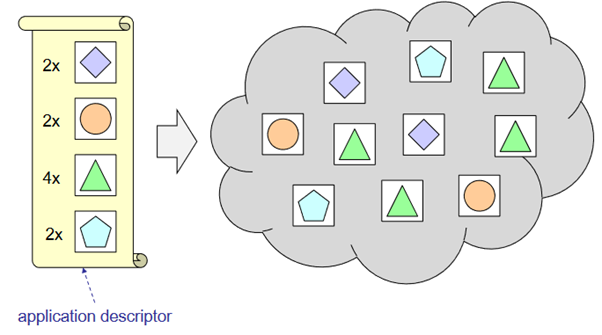
\includegraphics[width=0.9\textwidth]{imgs/kubernetes.png}
    \caption{Descrittore di un'applicazione per un cluster di contenitori \cite{cabibbo}}
    \label{fig:kubernetes}
\end{figure}
Kubernetes è un progetto open-source per la gestione di cluster di container. \\
I container sono raggruppati in pod (che sono ospitati su una o più macchine fisiche) ed ognuno di essi ha un suo indirizzo IP privato all’interno del cluster che gli consente di comunicare con gli altri pod. I container appartenenti allo stesso pod possono comunicare tra loro localmente senza dover passare attraverso un internet proxy, inoltre ogni pod può avere un proprio volume persistente a cui possono far riferimento tutti i container all’interno. I pod possono esistere solamente se al loro interno hanno almeno un container deployato, altrimenti vengono distrutti \cite{strachan-kubernetes}.\\
Kubernetes si occupa di monitorare i pod affinché venga garantito sempre il numero sufficiente di container attivi per una determinata applicazione, inoltre svolge anche funzionalità di service discovery per garantire la conoscenza dei servizi gli uni con gli altri permettendo inoltre l’esposizione di endpoint per poterli raggiungere dall’esterno.

\subsection{Apache Velocity}\label{velocity}
Velocity è un progetto open-source gestito dalla Apache Software Foundation basato interamente su Java. Permette la netta separazione tra il livello di business e presentazione di un'applicazione web secondo il pattern Model-View-Controller in \ref{fig:mvc}. \\
\begin{figure}[t]
    \centering
    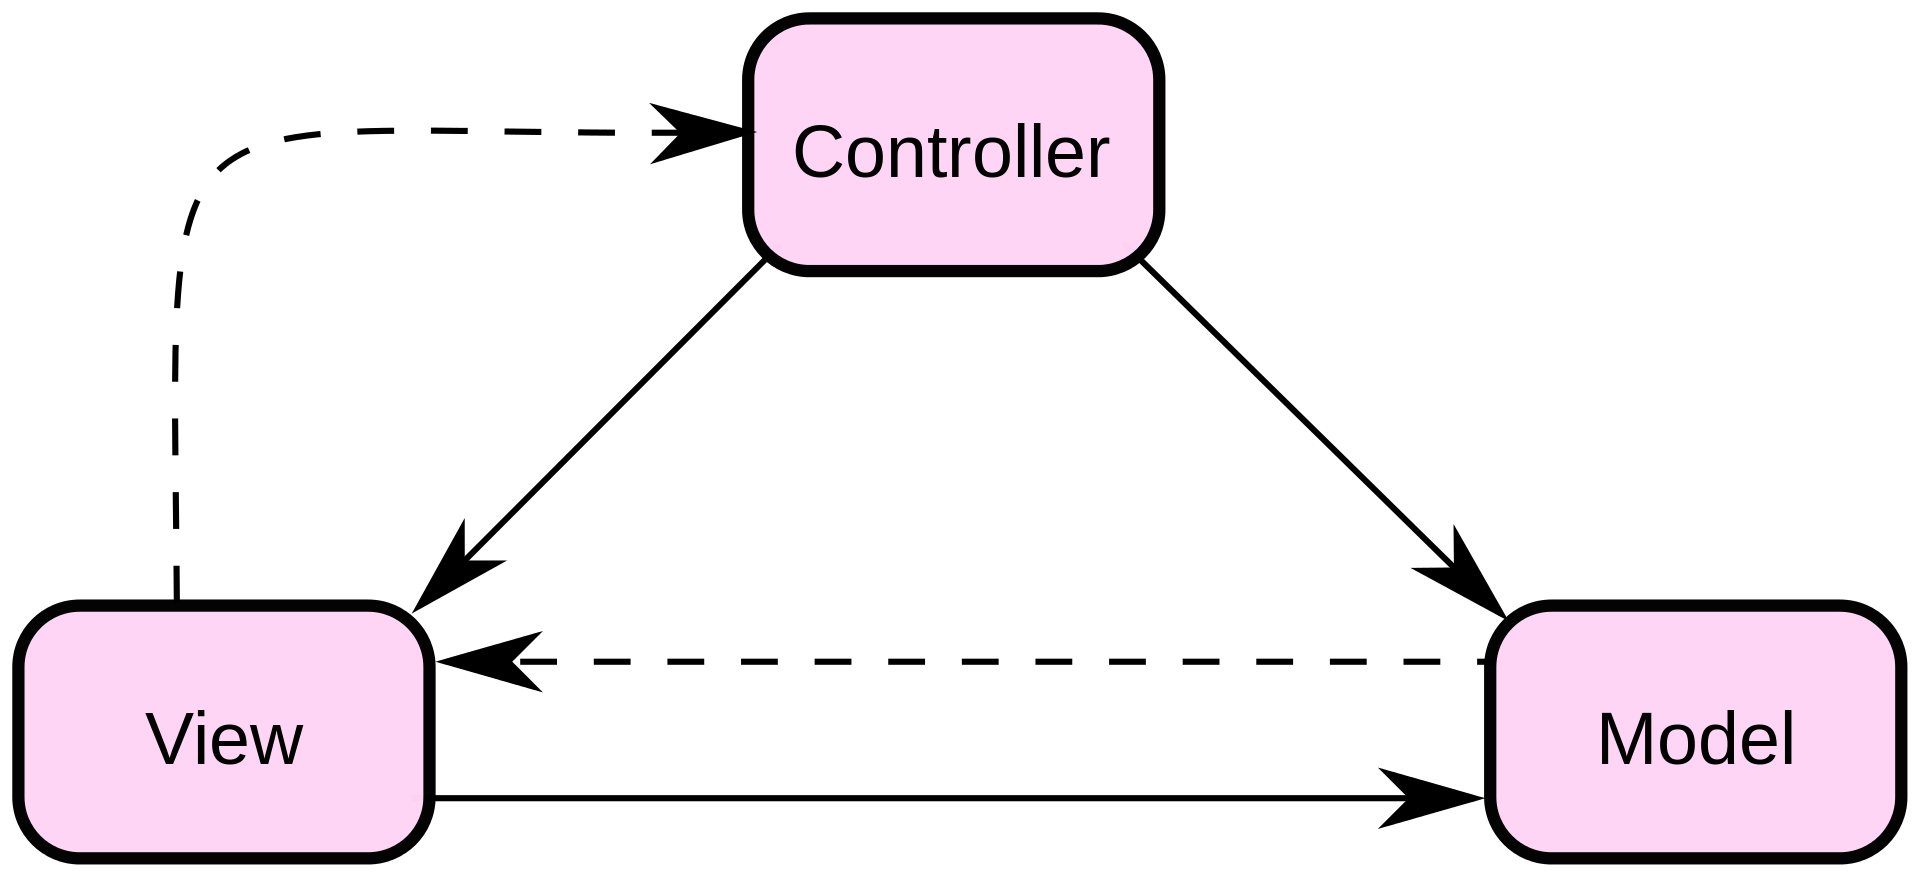
\includegraphics[width=0.9\textwidth]{imgs/ModelViewControllerDiagram2.png}
    \caption{Pattern Model-View-Controller}
    \label{fig:mvc}
\end{figure}
Velocity consente di introdurre dei contenuti generati dinamicamente all'interno di un template HTML utilizzando i comandi tipici di Java, permettendo quindi a sviluppatori e designer di agire in maniera indipendente e offrendo una migliore manutenibilità del codice.

\chapter{Contesto e requisiti}\label{requisiti}
La necessità di far conciliare processi già consolidati all’interno dell’azienda e l’applicazione di metodologie DevOps, ha necessariamente portato ad un’applicazione studiata appositamente per il caso in esame, e che quindi si discosta dall’applicazione ideale indicata dalla letteratura, ma che potrebbe essere applicabile ad aziende con le stesse caratteristiche e necessità.\\
Affinché un’organizzazione possa implementare in maniera efficace una soluzione DevOps, deve prima aver introdotto all’interno della propria filosofia di lavoro la metodologia Agile, infatti la prima non porterebbe alcun giovamento in un’azienda ancora legata all’approccio waterfall.

\section{Organizzazione Agile nelle grandi aziende}
L’applicazione della metodologia Agile non è un modello rigido che deve essere eseguito pedissequamente, altresì consiste in una serie di linee guida e principi da rispettare per migliorare l’efficienza del proprio team. Applicazioni dell’Agile possono variare da team a team, e comportano difficoltà che possono essere anche molto varie, perché dipendono soprattutto dall'attitudine delle persone coinvolte.\\
Considerato ciò, risulta evidente come una trasformazione Agile di una entità aziendale di grandi dimensioni sia necessariamente frutto di uno studio molto più complesso di quello che richiederebbe un singolo team o una startup, sia in termini di difficoltà di applicazione, che tempo in cui questa trasformazione venga resa effettiva e possa cominciare a restituire risultati concreti che possano essere misurati.
In un contesto simile, è facile che si sollevino degli scetticismi, in particolare da parte di quei dipendenti che vedono le proprie abitudini sconvolte da una tecnologia a cui ancora non sono riusciti ad avvicinarsi che improvvisamente ha portato a rendere obsoleta la loro esperienza nei vecchi processi aziendali.\\
Questo scetticismo generale alimentato dalla profonda riorganizzazione aziendale che l’Agile comporta, deve essere gestito adeguatamente dai manager, intesi come i diretti superiori, in rapporto stretto con i dipendenti e che quindi possono motivare, instradare ed essere in grado di mostrare la maggiore efficacia delle nuove metodologie ai propri dipendenti, mettendo in evidenza come un approccio simile aumenti la soddisfazione generale, non solo in termini di throughput, ma anche di esperienza lavorativa, creando un circolo virtuoso in cui azienda e dipendente sono entrambi vincitori.\\
La riorganizzazione prevede tra le altre cose:
\begin{itemize}
    \item la trasformazione dei team con conoscenze verticalizzate in team più cross-funzionali, composti da membri con conoscenze ed esperienze differenti tra loro così da favorire di conseguenza un trasferimento di conoscenze all’interno dei team. L’impatto di questa trasformazione si avverte soprattutto nel caso di grandi aziende, fortemente strutturate, che presentano dipartimenti verticalizzati e separati, a volte persino in edifici differenti, che necessariamente si trovano raramente a contatto gli uni con gli altri e che spesso comunicano tramite ticketing, richieste formali e processi rigidi, piuttosto che tramite un’interazione umana. Questo viola uno dei principi dell’Agile già descritto in \ref{agile}, ovvero: Gli individui e le interazioni, più che i processi e gli strumenti.
    \item L’ingresso nei team di un esperto Scrum (chiamato Scrum Master), che si preoccupi di garantire il rispetto delle cerimonie Agile come gli stand up meeting e le sprint reviews. Egli inoltre ha il ruolo di fungere da intermediario tra le richieste del manager e il team, affinché non si ritrovi sommerso da richieste che non siano in grado di gestire, garantendo perciò che il flusso di lavoro sia sempre ben definito ed organizzato \cite{scrum-ruoli}.
    \item L’insegnamento ai nuovi dipendenti delle pratiche Agile, in particolare agli Junior, così che possano da subito acquisire le migliori pratiche e possano diffonderle col tempo all’interno dell’azienda.
    \item Riorganizzazione dell’ufficio, in termini di dipartimenti e disposizione di scrivanie e open space, per garantire la massima comunicazione tra business, digital e in generale fra i vari dipartimenti, con l’introduzione di lavagne e strumenti per poter lavorare in modalità Agile.
\end{itemize}

\section{Requisiti funzionali}
Casi di studio hanno dimostrato che, nelle grandi organizzazioni, è più importante come i team collaborino tra loro per portare valore piuttosto che il metodo utilizzato dai singoli team \cite{gruver-agile} ed è per questo motivo che il processo DevOps deve coinvolgere tutte le componenti dello sviluppo software, facilitare la comunicazione tra le parti interessate e garantire un costante allineamento tra i team.\\
In aziende non nate come software house, dove la componente IT ha assunto importanza nell’ultimo decennio e dove i processi risultano molto strutturati, rigidi ed estremamente burocratizzati, la comunicazione solitamente avviene tramite l’utilizzo di richieste o l’aperture di ticket che si traducono in rallentamenti ed inefficienze, dal momento che l’intera catena può rimanere in attesa di un’approvazione da parte di un dipartimento differente. \\
Questa modalità non risulta Agile in quanto i team dedicati alla gestione della richiesta:
\begin{itemize}
    \item Non conoscono il contesto in cui la richiesta viene effettuata e devono impiegare del tempo per studiarlo
    \item Non si sentono coinvolti nel processo e pensano di essere un organo esterno che agisce in maniera indipendente servendo richieste (simile ad una modalità client-server)
    \item Non hanno come obiettivo la delivery del prodotto, ma solamente l’esecuzione del proprio task
    \item Percepiscono le richieste provenienti da altri team come un peso, avvertendo solo la propria mole di lavoro e non avendo una visione di quella degli altri team
\end{itemize}
Nonostante queste attività sembrino legacy\footnote{Termine inglese per “ereditati”: Utilizzato per definire un sistema obsoleto nei confronti degli standard tecnologici attuali.}, ancora oggi risultano imprescindibili per le grandi aziende che devono interfacciarsi con norme giuridiche e standard da rispettare, sia esterne (normativa GDPR, SOX compliance, ISO/IEC 27001) che interne.\\
Le attività relative al rispetto di norme e standard nazionali ed internazionali, per l’obbligo di essere revisionate e verificate da entità esterne unitamente all’alto livello di tracciabilità e documentazione imposto, solitamente, non risultano facilmente integrabili all’interno di un processo Agile. Le attività interne di solito riguardano il rispetto di certi standard imposti dall’azienda che di solito verificano la sicurezza e la gestione dei dati e delle risorse (come il rilascio in produzione o l’accesso alle macchine in particolari zone di sicurezza). \\
Ad esempio, un team addetto a queste verifiche potrebbe essere quello che si preoccupa di verificare che il codice non presenti falle di sicurezza, o che le comunicazioni tra le macchine avvengano su flussi e zone sicure, in modo da non esporre la rete aziendale a minacce o intrusioni. \\
Queste tipologie di controllo potrebbero essere rese molto più dinamiche e fluide se, ad esempio, una persona con competenze di sicurezza sedesse al tavolo con gli sviluppatori, fornendo la propria conoscenza come strumento per individuare le falle di sicurezza sul nascere, senza dover aspettare un feedback da un team esterno, o se persone con competenze di Operations sedessero al tavolo del team di sviluppo permettendo il rilascio in produzione senza la necessità di apertura di ticket o richieste formali.\\
Di conseguenza, valutando le necessità di adeguamento dei nuovi processi a quelli legacy e le difficoltà che si possono incontrare nell’applicare l’Agile su larga scala in termini di impatto sui dipendenti e sui processi, si è stabilito che una piattaforma DevOps debba mantenere e rispecchiare i ruoli di ciascun team coinvolto nello sviluppo e rilascio del software, integrandoli in un workflow attraverso l'utilizzo di strumenti di collaborazione dove ogni azione deve essere tracciata ed eseguita dal team preposto, attraverso la più stretta comunicazione possibile tra gli attori del processo.\\
L’obiettivo finale, oltre ad un incremento dell’efficienza complessiva e della competitività sul mercato in termini di costi, time to market e qualità del codice, deve essere anche il controllo sul processo, per assicurarsi che, rispetto alla conformità agli standard e ai processi in essere, non ci sia una regressione nei confronti dell’approccio tradizionale.

\section{Requisiti tecnici}\label{requisiti-tech}
I requisiti per l’applicazione di una piattaforma DevOps in un simile contesto è quello di poter mantenere un controllo completo sul processo, di garantire che determinate azioni possano essere svolte soltanto dai team predisposti a quella funzione, che ogni evento sulla piattaforma sia tracciato, che si possa tornare indietro in caso di fallimenti e che ogni passo del workflow sia ripetibile.\\
Per garantire tutte queste misure di sicurezza si è pensato all’utilizzo di un tracciatore di issue, ovvero un software che tenesse traccia degli sviluppi dalla stesa dei requisiti funzionali al rilascio del software, questo approccio ha inoltre permesso l’utilizzo delle pratiche Agile per la gestione del progetto, introducendo l’uso delle User Stories. L’utilizzo di uno strumento come questo, se da una parte rende il lavoro dello sviluppatore più legato al workflow e quindi con minore libertà di azione, permette un maggiore controllo generale e un unico punto di accesso su tutto il processo.\\
Un altro spunto d’interesse per lo studio di applicazione della DevOps è quello relativo allo sviluppo di software in maniera concorrente. I team di sviluppo possono essere formati da un elevato numero di programmatori, che devono poter essere in grado di lavorare in maniera indipendente e concorrente. Per far fronte a ciò esistono diversi modelli di Git workflow applicabili, per questo contesto aziendale in cui i team possono essere di grandi dimensioni e c’è bisogno di un allineamento tra il tracciamento degli issue e le modifiche al software, il modello che è risultato più robusto e compatibile è il Gitflow workflow \cite{driessen-gitflow}.\\
Un numero elevato di sviluppatori e, di conseguenza, modifiche al codice che possono essere eseguite in parallelo, porta alla necessità di mantenere frequentemente allineati gli ambienti con le versioni del codice, ciò si traduce nell’uso di commit frequenti e regolari. Questa tipologia di approccio, chiamata in letteratura con il nome di Continuous Integration, ha bisogno di un software adeguato, che possa essere raggiungibile da qualsiasi punto dell’infrastruttura, con la funzione di “mente” di tutta la piattaforma DevOps.


\chapter{Parti coinvolte nel processo DevOps}\label{teams}
In \ref{devops} si è spiegato come la DevOps non sia solamente un’automatizzazione dei processi, ma  anche e soprattutto una filosofia che coinvolge i team e li spinge a lavorare in maniera più agile, per questo è utile definire quali sono i team IT che vengono coinvolti all’interno del processo, illustrandone brevemente i cambiamenti che porta l’adozione di una piattaforma DevOps nei confronti del tradizionale metodo a cascata.\\
In un contesto aziendale di grandi dimensioni, implementare uno stato dell’arte di una piattaforma DevOps risulta complesso in breve tempo, per questo è stato introdotto il concetto di “champion”, ovvero di esperto di un determinato settore che fornisce supporto al team di un altro settore.

\section{Team Funzionale}
Il team funzionale è normalmente composto da componenti del business e componenti dell’IT, è incaricato di raccogliere i requisiti richiesti da chi commissiona il software (che può essere sia interno che esterno all’azienda) e trasformarli in casi d’uso da sottomettere al team di sviluppo.\\
Nell’approccio a cascata, questa attività viene eseguita all’inizio del ciclo di sviluppo del software, utilizzando invece un approccio agile, un team funzionale può facilmente introdurre nuovi casi d’uso a seconda delle esigenze del business. Facendo parte del processo DevOps, un membro del team funzionale può loggarsi al sistema della raccolta dei requisiti ed inserire il nuovo caso d’uso, che verrà sviluppato durante lo sprint successivo.

\section{Team di Sviluppo}
Il team di sviluppo è la “mano”, come suggerisce il nome, di tutto il processo di sviluppo del software, è lui che si occupa della trasformazione dei casi d’uso in effettive funzionalità del prodotto. Inoltre è incaricato dello sviluppo e dell’esecuzione dei test preliminari sul codice per verificare la correttezza dello stesso.\\
Nell’approccio tradizionale riceve i requisiti dal team funzionale ed inizia la fase di sviluppo finché tutti i casi d’uso non sono completati, lasciando il compito di testare il software al team di QA e di UAT.\\
Con l’introduzione della piattaforma DevOps, gli sviluppatori, supportati da tecnologie come il modello di Gitflow e la Continuous Integration, hanno la possibilità di avere un maggiore controllo sulle modifiche al codice e sui rilasci eseguiti ad ogni sprint. Inoltre è il processo stesso a guidare lo sviluppatore, che ha ridotto al minimo le attività secondarie e che quindi può dedicarsi completamente alla scrittura del codice.
Quindi il team di sviluppo può lavorare in sprint producendo codice funzionante e testato, non lasciando mai il software in una situazione di non consistenza. Così una modifica richiesta dal business può essere rapidamente analizzata dal team funzionale e passata al team di sviluppo che nell’arco della durata di uno sprint, è in grado di includerla nella prossima release del software.

\section{Team di Quality Assurance}
Nel sistema waterfall, il team di QA interviene nella fase immediatamente successiva a quella dello sviluppo del software. Il team degli sviluppatori rilascia il software in un ambiente di testing e il team di QA provvede ad effettuare una serie di test a scatola chiusa, che non prevedono cioè la conoscenza del pacchetto applicativo. I risultati dei test ed eventuali bachi vengono segnalati al team di sviluppo.\\
Con l’utilizzo della piattaforma DevOps, il team di QA lavora a stretto contatto con il team degli sviluppatori, per esempio sedendo allo stesso tavolo, per l’esecuzione di test di qualità sul prodotto, verificando che il software soddisfi i requisiti imposti dal business e che le nuove modifiche non introducano delle regressioni, ovvero dei malfunzionamenti introdotti dalle nuove funzionalità implementate.\\
La maggior parte del codice deve essere verificato tramite l’utilizzo di test automatici integrati direttamente nel processo di Continuous Integration, compreso il rilascio del prodotto nell’ambiente di testing.\\
Il test da parte del team di QA o di UAT, avviene per singola US, essendo nel modello Agile la singola US la minima quantità di funzionalità sviluppata, testata e rilasciabile. 

\section{Team di User Acceptance Test}
Il team di UAT è forse quello che risulta meno coinvolto nel processo DevOps, in quanto le sue attività rimangono simili a quelle dell’approccio waterfall.
Il team di UAT ha il compito di verificare la funzionalità del software eseguendo dei test in un ambiente che è quanto più possibile simile a quello di produzione. Gli User Acceptance Test rispecchiano il punto di vista dell’utente, ed in pratica sono la dimostrazione del funzionamento del sistema più vicina al mondo reale.\\
Nel processo DevOps il processo è semplificato dall’automatismo garantito dalla piattaforma. Quando il software supera i test eseguiti dal team di QA, esso viene rilasciato sull’ambiente dedicato agli UAT, quindi il team preposto esegue i test e segnala eventuali problemi o dà la propria approvazione per il passaggio del software nell’ambiente di produzione.
\section{Team di Operations}
Nel mondo waterfall, le attività eseguite dal team di Operations consistono nell’esecuzione di operazioni descritte in documenti o manuali dettagliati, che elencano una serie di task da eseguire per il rilascio del software nell’ambiente di produzione, lasciando il più possibile il sistema a “scatola chiusa”.\\
Lo scopo principe del processo DevOps è quello di avvicinare il più possibile le realtà dello sviluppo e delle Operations per rendere i rilasci il più possibile frequenti e corretti.
Con l’introduzione del modello DevOps, il team di Operations riceve il software al termine del workflow, ovvero quando tutti gli step precedenti sono stati completati e superati, come nell’approccio waterfall, ma a differenza di esso, utilizzando la metodologia di CI/CD, queste operazioni possono arrivare ad essere eseguite più volte nello stesso giorno.\\
Per questo motivo la massima standardizzazione e, di conseguenza, automazione del processo di rilascio, è ciò che deve essere perseguito dalla soluzione DevOps, permettendo al team di Operations di dedicare il minor tempo possibile all’esecuzione dei rilasci e permettendo così una maggiore attenzione sulla gestione dei sistemi in produzione.\\
L’applicazione della metodologia DevOps prevede la presenza di un membro del team di Operations al tavolo dello sviluppo e il passaggio di conoscenze fra sviluppatori e Operations. Questo porterebbe al vantaggio di una maggiore consapevolezza del software che viene rilasciato da parte delle persone di Operations e una maggiore consapevolezza dei rischi associati ad un rilascio in un ambiente di produzione da parte degli sviluppatori, avvicinando definitivamente i due mondi e permettendo rilasci più robusti e frequenti. \\
Nel caso di fallimenti nel processo DevOps, il team di Operations può intervenire manualmente per garantire il corretto funzionamento dell’infrastruttura, inoltre ha il compito di segnalare al team di DevOps eventuali malfunzionamenti e bug nel processo.

\section{Team di Security}
Il team di sicurezza si occupa di testare la resistenza del codice tramite penetration test per rilevare eventuali vulnerabilità.\\
Nell’approccio tradizionale, esso opera in maniera indipendente dal team di sviluppo: riceve il pacchetto software, effettua i test e fornisce il suo feedback. Il tema della sicurezza pertanto viene valutato solo al completamento dello sviluppo ed un eventuale vulnerabilità, per essere risolta, comporta un ritardo e un costo notevoli nella consegna del prodotto finale.\\
Scopo della DevOps, che a seconda dell’attenzione posta sul tema della security in letteratura spesso prende il nome di DevSecOps \cite{myrbakken-devsecops}, è quello di valutare la sicurezza del prodotto prima possibile, spostando tutti i controlli, di sicurezza o meno, anticipandoli quanto più possibile nel ciclo di vita del processo, in maniera tale da minimizzare ogni riciclo sullo sviluppo del software successivo alla rilevazione di un security flaw. Ciò si ottiene attraverso l’integrazione di strumenti automatizzati di sicurezza statica e dinamica (SAST e DAST) all’interno del processo DevOps e alla presenza di un esperto di sicurezza (chiamato “security champion”) al tavolo dello sviluppo.\\
In questo modo, tramite lo scambio di conoscenze tra sviluppatori ed esperti di sicurezza, il codice può essere da subito implementato secondo elevati standard di sicurezza, così che il prodotto, il team e il processo stesso ne possano beneficiare.

\section{Team di DevOps}
Il team di DevOps è il “direttore d’orchestra” di tutto il processo. È composto da tecnici con conoscenze nell’ambito dello sviluppo e delle operations e collabora con i due team per apportare migliorie al processo.\\
Occupa una posizione trasversale rispetto agli altri team, avendo il compito di verificare la correttezza del processo di DevOps e di intervenire laddove si rendano evidenti errori o su segnalazione delle altre parti coinvolte, così da garantire la maggiore fluidità possibile.\\
Inoltre è responsabile dell’onboarding di ogni nuovo sistema all’interno della piattaforma realizzata, disegnando il processo in collaborazione con i diversi team coinvolti e implementandone la soluzione.


\chapter{Analisi e scelta dei software}\label{software}
Nel corso del progetto ho preso parte alle fasi finale dei processi di decisione, assieme agli ingegneri Alessandro Casula e Massimiliano Romano, dove erano già stati definiti i componenti, ma non gli strumenti da utilizzare. Durante le fasi di analisi è emerso spesso il contrasto nella scelta di software open source o proprietario, perciò ho inserito un breve paragrafo di ricerca sulle motivazioni che possono portare a sceglierne uno nei confronti dell'altro.  In questo capitolo sono elencati i risultati delle sopracitate riunioni e le conclusioni che ne sono state tratte.

\section{Confronto software open-source e proprietario}
In questo paragrafo vengono esposti i pro e i contro nell’utilizzo di software aperto e proprietario \cite{opensource-vs-proprietary}. In particolari sono stati considerati i seguenti aspetti nell’analisi fatta: costo, supporto applicativo, documentazione, intervento sui bug e sulla sicurezza, complessità d’uso, integrazione con altri sistemi e la libertà derivante dal loro utilizzo.\\
Costo e supporto applicativo:
\begin{itemize}
    \item \emph{Open-source}: i software open source solitamente presentano costo nullo a fronte di un supporto che è costituito dalla community, che risponde tramite l’utilizzo di forum e siti di Question Answering, ma che ovviamente non è in grado di offrire la stessa assistenza di un servizio a pagamento.
    \item \emph{Proprietario}: i software proprietari hanno un costo dettato dal numero di licenze che è necessario utilizzare, che possono basarsi ad esempio sul numero di utenti o su una durata temporale. Solitamente nel prezzo è compreso il supporto da parte di personale altamente qualificato per intervenire in caso di necessità. L’utilizzo di numerosi software proprietari introduce una maggiore complessità data dalla necessità pratica di gestire i differenti sistemi di tariffazione e licenze.
\end{itemize}
Documentazione:
\begin{itemize}
    \item \emph{Open-source}: i software open-source presentano una documentazione di norma più scarna o non aggiornata rispetto ad un software proprietario. Essendo dei progetti che vengono sviluppati da persone che non traggono alcun profitto, l’importanza data alla presenza di manuali è messa in secondo piano o addirittura non è contemplata.
    \item \emph{Proprietario}: la documentazione è estremamente dettagliata e fornita di manuali ed esempi di utilizzo che vengono aggiornati con l’avanzare del software. Inoltre per casi in cui la documentazione non sia sufficiente è possibile chiedere aiuto al supporto applicativo.
\end{itemize}
Gestione dei bug e sicurezza:
\begin{itemize}
    \item \emph{Open-source}: la trasparenza del codice open source garantisce che un bug possa essere risolto in tempi brevi che nella maggior parte dei casi sono più brevi rispetto ad un software proprietario \cite{opensource-vs-proprietary-bugs}, questo perché la presenza di un numero elevato di sviluppatori riduce sensibilmente la possibilità che la soluzione di un bug si protragga nel tempo. Questo punto, sebbene dovrebbe rappresentare sempre un vantaggio, espone l’azienda ad un maggiore rischio perché un bug è molto probabile sia noto al pubblico, e degli utenti maligni potrebbero sfruttarlo per arrecare danno all’azienda.
    \item \emph{Proprietario}: un software proprietario può ricevere segnalazioni sulla presenza di bug, ma la gestione di quella problematica potrebbe non essere quella a più alta priorità e il bug potrebbe presentarsi per una durata maggiore prima di venir risolto. La chiusura del software inoltre non permette di poter accedere al codice sorgente al personale esterno all’azienda che fornisce il software. Per quanto concerne la sicurezza, i software proprietari fanno dell’opacità del proprio codice un punto di forza, ma in caso una falla di sicurezza venisse scoperta, i tempi per porre rimedio sono, per le ragioni descritte prima, maggiori rispetto ad un software open source.
Complessità di utilizzo:
\end{itemize}
Complessità di utilizzo:
\begin{itemize}
    \item \emph{Open-source}: un software open-source, per le ragioni elencate precedentemente, quali la mancanza di un supporto e di una documentazione efficaci, risultano più complessi da gestire e da utilizzare rispetto alla controparte. Perciò si deve introdurre un costo necessario al training dei team interni all’utilizzo di quel sistema oppure pagare un fornitore esterno per poter contare su un team in grado di utilizzare quel prodotto.
    \item \emph{Proprietario}: un software proprietario fornisce solitamente un software “pronto all’uso”, ovvero che possa essere utilizzato senza avere conoscenze tecniche approfondite, accompagnato da una grafica gradevole ed intuitiva che ne facilita l’uso.
\end{itemize}
Integrazione con altri sistemi:
\begin{itemize}
    \item \emph{Open-source}: un software open-source potrebbero avere un elevato grado di integrazione con altri strumenti, grazie alla trasparenza del codice descritta precedentemente.
    \item \emph{Proprietario}: un software proprietario solitamente si integra perfettamente con altri software della stessa azienda produttrice (come ad esempio Microsoft Outlook e Skype). Essendo nell’interesse delle aziende essere il più flessibili possibile, anche l’integrazione con software open source rappresenta un obiettivo da perseguire.
\end{itemize}
Libertà di utilizzo:
\begin{itemize}
    \item \emph{Open-source}: un software open-source non è legato a nessuna azienda e, una volta imparato ad utilizzare e conoscere,
    \item \emph{Proprietario}: un software proprietario implica una relazione continua con il fornitore e, più il software ha responsabilità all’interno del progetto, più è complicato cambiarlo con un prodotto concorrente.
\end{itemize}

\section{Software di tracciamento issue}
Un processo DevOps può avere differenti requisiti di controllo, nel caso di un sistema aziendale questi requisiti sono molto stringenti. Visto che la facilità di gestione e controllo di un sistema è inversamente proporzionale ai punti accessibili dall’esterno, è preferibile utilizzare un unico punto di accesso da cui sia possibile gestire l’intero ciclo di vita dello sviluppo software, dalla scrittura della user story fino al suo rilascio in produzione.
Esistono numerosi strumenti che permettono di mantenere un tracciamento di issue, che possono variare dall’implementazione di nuove funzionalità alla risoluzione di bug o all’aggiornamento dell’interfaccia grafica. Le informazioni utilizzate per il tracciamento sono salvate all’interno di un database, con un codice riconoscitivo dell’issue, la sua gravità, una breve descrizione, opzionalmente indicazioni per poter riprodurre l’errore, chi ha segnalato il problema e lo sviluppatore che ci sta lavorando.
Dopo un’analisi sui principali software per il tracciamento di bug e issue, i seguenti quattro sono i candidati per la gestione della piattaforma DevOps, sia open source che con licenza proprietaria:
\begin{enumerate}
    \item Bugzilla
    \item Jira
    \item Mantis
    \item Pivotal Tracker
\end{enumerate}

\subsection{Bugzilla}
Bugzilla è uno dei primi software di bug-tracking sviluppato dal team di sviluppo di Mozilla Firefox, scritto in Perl, segue la stessa filosofia open-source. Per poter essere utilizzato necessita di un web server (tipicamente Apache) e un DBMS. Può essere utilizzato non solo per il tracciamento dei bug, ma anche per la gestione delle richieste di sviluppo di nuove features.
\begin{figure}
    \centering
    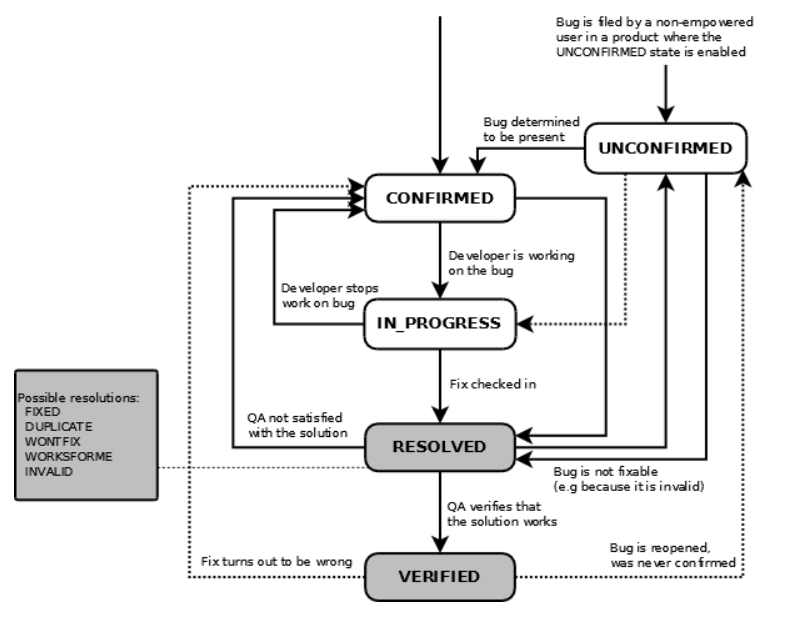
\includegraphics[width=0.9\textwidth]{imgs/bugzilla.png}
    \caption{Workflow di un bug in Bugzilla \cite{bugzilla-doc}}
    \label{fig:bugzilla}
\end{figure}

\subsection{Jira}
Jira è un software che permette il tracciamento di issue e bug, scritto in Java, di proprietà di Atlassian. Tra le varie funzionalità integra anche strumenti per la gestione Agile dei progetti, come la possibilità di definire bacheche Kanban e Scrum con task direttamente collegati alle issue. Esiste in due versioni principali, Cloud (principalmente per le funzionalità Agile) e Server, nel secondo caso ha bisogno di un DBMS su cui memorizzare le informazioni relative alle issue. Inoltre permette di modificare i workflow delle issue per adattarli al metodo di lavoro del team e di definire dei report Agile personalizzati.
\subsection{Mantis}
Mantis è un software open source sviluppato da Victor Boctor, scritto in PHP, come per Bugzilla, anche lui necessita solamente di un web server e di un DBMS per poter funzionare. Il principio di funzionamento è pressoché identico al diretto concorrente open source, ma i due sistemi presentano sottili differenze che li rendono più o meno applicabili a seconda delle esigenze.
\subsection{Pivotal Tracker}
Pivotal Tracker è un software di tracciamento issue scritto in Ruby di proprietà di Pivotal, include strumenti di gestione dei progetti in Agile e possibilità di personalizzazione dei workflow. Come Jira, consente una gestione a 360 gradi del progetto, dalle roadmap di sviluppo all’assegnazione dei task.
\subsection{Confronto}
A fronte di queste considerazioni, di seguito una tabella riassuntiva dei pro e contro dei differenti software:
\begin{figure}
    \centering
    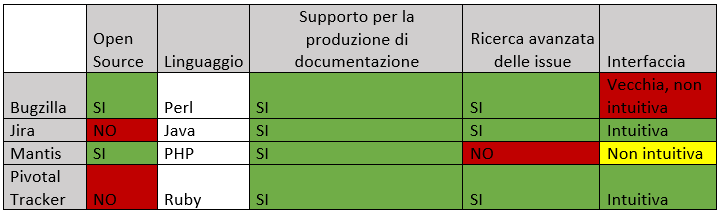
\includegraphics[width=0.9\textwidth]{imgs/confronto-sw-issue.PNG}
    \caption{Confronto tra i sw di issue tracking}
    \label{fig:confronto}
\end{figure}
In conclusione, si è deciso di utilizzare Jira come sistema di gestione dell’intero processo DevOps, in particolare per la presenza di API che permettono di integrarsi con numerosi altri strumenti di CI/CD, per la possibilità di gestire team non solo in termini dello sviluppo di codice, ma anche di assegnazione dei task, per l’interfaccia intuitiva, la possibilità di effettuare ricerche avanzate all’interno del database, la presenza di un buon supporto sul prodotto.\\
All’interno del progetto, l’uso di Jira è customizzato sulla base delle esigenze di progetto, in particolare l’obiettivo ricercato è quello di essere agnostico ai sistemi che lo utilizzeranno come piattaforma DevOps: al centro di tutto vi è l’\emph{issue}, che può essere di vario genere, ma che generalmente consiste in un elenco di requisiti, scritti da analisti funzionali del business, che devono essere implementati nel codice dagli sviluppatori. Un issue può essere composto da più \emph{subtask}, che sono una riduzione minima delle operazioni che devono essere eseguite per completare i requisiti e che vanno ad impattare un solo componente del software, quando tutti i subtask sono dichiarati completati, allora la issue è pronta per essere testata e rilasciata. Quando le issue create all’interno dello sprint vengono completate, viene creato un oggetto release, che generalmente funge da contenitore e comprende tutte le issue etichettate con la stessa versione. Un’issue di test si occuperà della scrittura dei test da eseguire sul codice relativo (test di non regressione o end to end) ad una certa release, che possono essere sia eseguiti in automatico tramite delle pipeline o manualmente dagli sviluppatori. La release poi passerà delle fasi di test di integrazione e deploy su ambienti via via più simili a quello di produzione, fino al vero e proprio rilascio nell’ambiente di produzione.

\section{Software di wiki}
Il software per mantenere la documentazione del progetto deve rispettare tre requisiti principali:
\begin{itemize}
    \item Interfaccia più intuitiva possibile
    \item Integrazione con Jira
    \item Possibilità di inserire divisioni per progetti e ruoli
    \item Sintassi tramite markdown
\end{itemize}
All’interno di questa wiki deve essere creato un folder per ogni progetto che utilizzerà la piattaforma DevOps e deve essere acceduto dagli utenti coinvolti nei progetti con i relativi permessi. \\
La struttura di un folder di un generico progetto è così composta:
\begin{itemize}
    \item Requisiti funzionali
    \item Documentazione generica, tecnica o non (con relative sottocartelle)
    \item Note di rilascio (generate automaticamente in uno step della pipeline di DevOps)
\end{itemize}
Trattandosi di uno strumento molto utilizzato nell’enterprise e facente parte della stessa suite di Jira, avendo quindi delle API built-in per poter interfacciarvisi, Confluence è stato scelto come strumento di documentazione.

\subsection{Confluence}
La versione server richiede la presenza di un database che possa fare da filesystem per le pagine inserite, strutturate ad albero, dove la radice è rappresentata da uno \emph{space} e i nodi sono \emph{pages}, una page può averne altre sotto di sé e quindi permettere di raggrupparle per argomento, ma può comunque contenere del testo. Le pagine possono essere modificate con un semplice editor di testo e possono contenere tabelle, grafici, immagini, etc.

\section{Software per il controllo di versione}
Per versioning del codice sorgente si intende la possibilità di tenere uno storico delle modifiche effettuate all’interno di file e cartelle, così che nel caso un cambiamento non abbia portato agli effetti sperati o non sia più necessario, possa essere annullato.\\
Per il versioning del codice sorgente le seguenti due tecnologie sono state prese in considerazione:
\begin{itemize}
    \item Subversion 
    \item Git
\end{itemize}
Entrambe le tecnologie ottengono lo stesso risultato, ma in maniera differente, pertanto è necessaria un’analisi per stabilire quali tra le due sia quella più efficace all’interno del contesto di progetto.

\subsection{Subversion}
È un software open source per il controllo di versione sviluppato dalla Apache Software Foundation. Prevede la presenza di un server centrale su cui è contenuta la versione “stabile” del codice all’interno di un repository; per implementare delle modifiche un utente deve scaricare una copia di lavoro del repository sulla propria macchina, scrivere il codice e inviare la modifica al server centrale con il comando commit. Per questa ragione viene descritto come un sistema centralizzato. Permette la presenza dei branch, ovvero delle “copie” del repository dove un utente può implementare le proprie modifiche senza interferire col lavoro degli altri sviluppatori, mantenendo comunque il codice visibile agli altri membri del team.
\begin{figure}
    \centering
    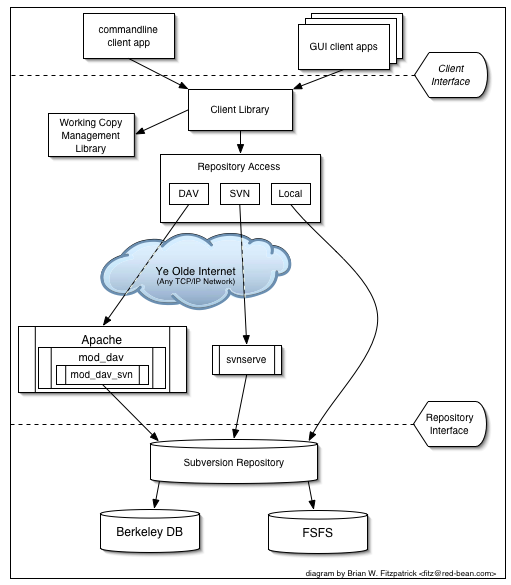
\includegraphics[width=0.9\textwidth]{imgs/subversion.png}
    \caption{Architettura di Subversion \cite{svn-docs}}
    \label{fig:subversion}
\end{figure}
\subsection{Git}
È un software per il controllo di versione open source sviluppato da Linus Torvalds. Si differenzia da Subversion principalmente per la sua natura distribuita: i commit e i branch possono essere eseguiti sul repository locale dell’utente, che è una copia del repository remoto (comprensiva di tutta la history). L’utente, quando lo desidera può allineare il repository locale a quello remoto gestendo eventuali modifiche concorrenti, chiamati conflitti.
\begin{figure}
    \centering
    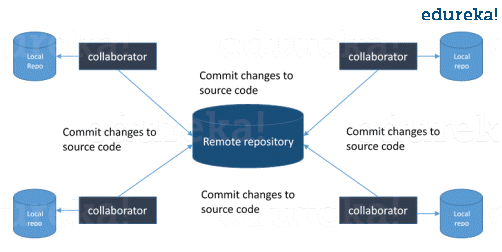
\includegraphics[width=0.9\textwidth]{imgs/git.png}
    \caption{Architettura di Git \cite{git-docs}}
    \label{fig:git}
\end{figure}
\subsection{Confronto}
La maggiore velocità e libertà di azione offerta da Git agli sviluppatori, nonché l’essere l’ambiente nativo di applicazione di Git Workflow, ha fatto ricadere la scelta su quest’ultimo. Uno sviluppatore può effettuare le modifiche direttamente sulla propria macchina senza il bisogno di avere una connessione internet per poter contattare il server centrale, di conseguenza Git è anche più resiliente ai guasti, infatti permette di lavorare anche nel caso ci sia un guasto sulla rete o sul server, inoltre il codice con la history dei commit può essere sempre recuperato da un repository locale di un membro del team.
\subsection{Bitbucket}
Avendo già scelto Jira e Confluence dalla suite Atlassian, per praticità si è scelto Bitbucket, software web-based per l’hosting di progetti che utilizzano Git o Mercurial, di proprietà della stessa azienda.\\
Fornisce un’interfaccia grafica con funzionalità intuitive per la gestione del repository, permette di effettuare dei commit minimali direttamente da browser, senza necessità di clonare il repository per effettuare piccole modifiche, inoltre si integra nativamente con gli altri strumenti di Atlassian e consente la comunicazione con il software di CI tramite delle API.

\section{Software per CI/CD}
Come descritto al paragrafo 2.2.1, la Continuous Integration (CI) è un approccio dell’ingegneria del software dove l’obiettivo è quello di fare in modo che ogni modifica al codice non porti ad una regressione del software.\\
Ogni sviluppatore può allineare il proprio repository anche più volte al giorno, essendo sicuro che, nel caso ci sia un errore, questo venga rilevato in tempi brevi e facilmente individuato. Quindi ogni commit su Git deve scatenare una sequenza di eventi che testino in automatico la modifica. Tali azioni devono essere gestite e coordinate da un software di Continuous Integration.
\begin{figure}
    \centering
    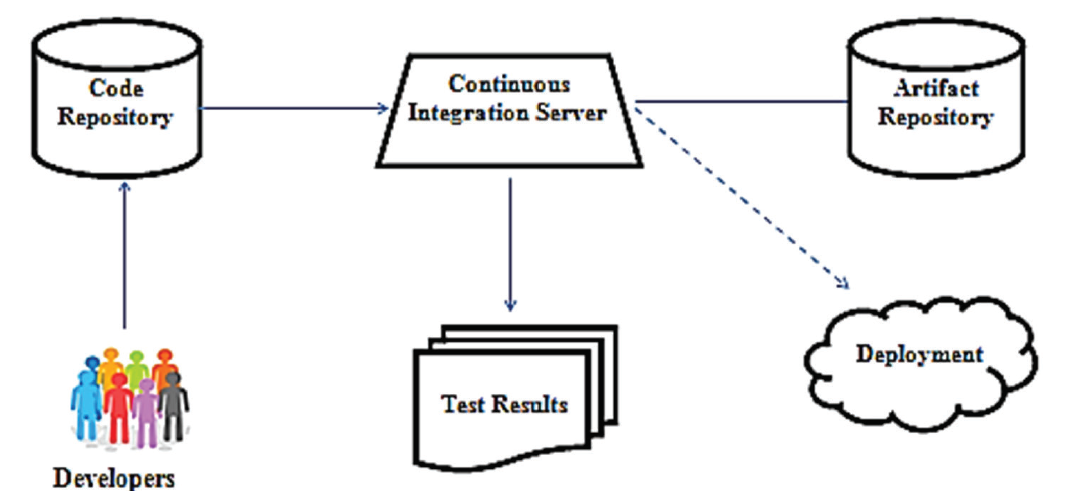
\includegraphics[width=0.9\textwidth]{imgs/ambiente-ci.png}
    \caption{Ambiente di Continuous Integration \cite{ci-env}}
    \label{fig:ambiente-ci}
\end{figure}

\subsection{Jenkins}
Jenkins (precedentemente Hudson) è un software open source di Continuous Integration sviluppato in Java e scritto da Kohsuke Kawaguchi nel 2011, viene eseguito su un servlet container come Apache Tomcat ed è utilizzabile da un’interfaccia web. Permette l’installazione di numerosi plugin per integrarlo con tool esterni, garantendo un’alta versatilità.
\begin{figure}
    \centering
    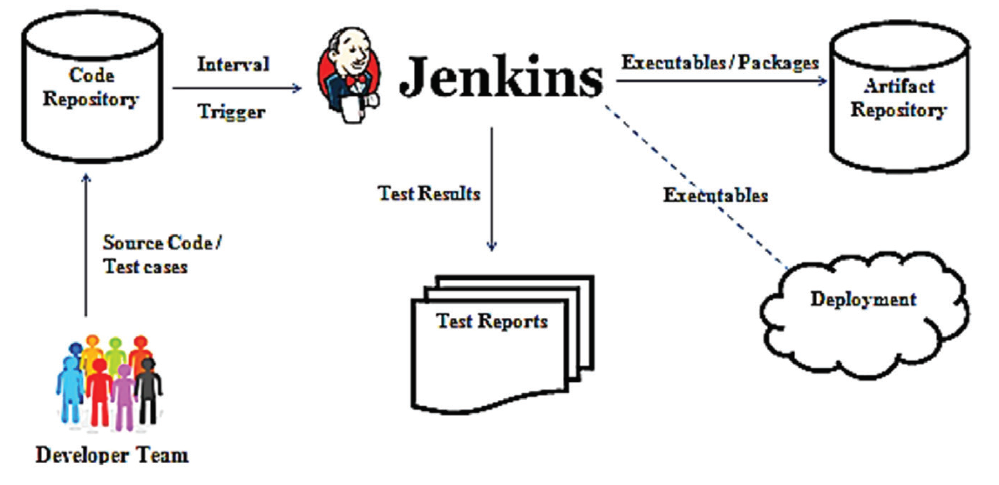
\includegraphics[width=0.9\textwidth]{imgs/ambiente-ci-jenkins.png}
    \caption{Ambiente di CI con Jenkins \cite{ci-env}}
    \label{fig:ambiente-ci-jenkins}
\end{figure}
Il trigger per l’esecuzione nativamente può consistere in diverse azioni, che possono essere estese tramite i plugin.\\ 
I trigger utilizzati internamente al progetto sono:
\begin{itemize}
    \item un commit su Git
    \item la creazione di un task su Jira
    \item il termine di un’altra pipeline
\end{itemize}

\begin{figure}[H]
    \centering
    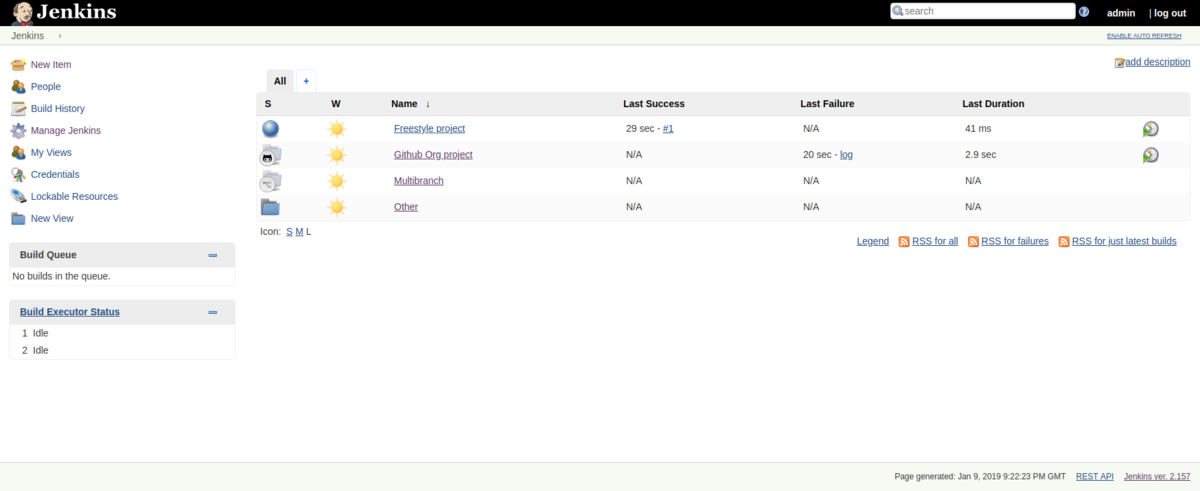
\includegraphics[width=0.9\textwidth]{imgs/jenkins-gui.png}
    \caption{Interfaccia web di Jenkins}
    \label{fig:jenkins-gui}
\end{figure}
Una pipeline è una sequenza di \emph{stadi} che devono essere eseguiti in sequenza, se uno step fallisce l’intera pipeline viene interrotta. Questo permette allo sviluppatore di individuare rapidamente errori nel codice o nel processo.\\
Le pipeline possono essere di due tipi, dichiarative o definite come script \cite{jenkins-docs}:
\begin{itemize}
    \item le pipeline \emph{dichiarative} hanno una sintassi più ad alto livello e consentono di scrivere rapidamente pipeline più semplici.
    \item le pipeline definite come \emph{script} sono scritte in Groovy (un linguaggio di scripting per la piattaforma Java e pertanto offre le stesse funzionalità) e di conseguenza, offrono la flessibilità di un linguaggio di programmazione ad oggetti.
\end{itemize}
Per lo scopo della piattaforma, le pipeline sono definite in Groovy, per offrire la maggiore flessibilità possibile.

\begin{comment}
\section{Strumento per l'automazione dello sviluppo}
Parte fondamentale nell’applicazione della Continuous Integration è la build automatica delle modifiche introdotte dagli sviluppatori. Queste build, scatenate dalle pipeline di Jenkins, devono essere eseguite tramite uno strumento di build automation.
I principali strumenti per la build automation in ambiente Java sono \cite{build-tools}:
\begin{itemize}
    \item Apache Ant con Ivy
    \item Apache Maven
    \item Gradle
\end{itemize}
Lo scopo di questi strumenti lo stesso, guidare la compilazione del codice durante tutto il suo ciclo di build, che tendenzialmente comprende questi step principali:
\begin{itemize}
    \item Analisi statica del codice
    \item Esecuzione di test unitari
    \item Creazione dell’artefatto (il software compilato e pronto per essere eseguito)
\end{itemize}


\subsection{Apache Ant con Ivy}
Apache Ant è un progetto nato nel 2000, prevede l’esecuzione di step definiti in un documento chiamato \emph{build.xml}, dove sono elencati a grana fine i passaggi da eseguire per generare l’artefatto. La gestione delle dipendenze da remoto viene fatta tramite Ivy, che si occupa di scaricare le librerie ed i plugin definiti in un file chiamato \emph{ivy.xml}.
\subsection{Apache Maven}
Apache Maven è un progetto nato nel 2004 per intervenire sulle mancanze di Apache Ant e semplificare alcuni step che si trovano ripetuti in ogni sviluppo software. Maven comprende il proprio gestore di dipendenze, che soddisfa tramite la consultazione di un file di properties chiamato \emph{pom.xml} (Project Object Model).
\subsection{Gradle}
Gradle è uno strumento open source che prende ispirazione dalle precedenti esperienze di Apache Maven e Apache Ant per offrire un prodotto più efficiente. Lo stato desiderato del progetto è definito in un file chiamato \emph{build.gradle}, in cui sono descritti i task in un linguaggio domain-specific\footnote{Linguaggio di programmazione dedicato a specifici problemi di un dominio.} basato su Groovy, di più facile lettura e dimensione rispetto ad un file XML. I task non devono essere eseguiti in maniera sequenziale, ma hanno una struttura definita da una clausola “dependsOn”, andando a costruire un grafo diretto aciclico.\\
Di seguito un esempio di file \textbf{build.gradle}:
\begin{verbatim}
    task hello {
        doLast {
            println 'Hello world!'
        }
    }
    task intro {
        dependsOn hello
        doLast {
            println "I'm Gradle"
        }
    }
\end{verbatim}

%\begin{figure}
%    \centering
%    \includegraphics[width=0.9\textwidth]{}
%    \caption{Esempio di file build.gradle}
%    \label{fig:build-gradle}
%\end{figure}

\subsection{Confronto}
In questo caso la scelta è stata guidata soprattutto dalla maggiore conoscenza complessiva di Apache Maven all’interno del team di sviluppo. La piattaforma DevOps tuttavia è stata pensata per poter utilizzare una nuova tecnologia con un intervento poco invasivo, così da dare ai programmatori un’alta flessibilità nei confronti delle loro esigenze.\\
Apache Maven è uno strumento di gestione di progetti software che ha lo scopo di semplificare il processo di build del codice. 
Tra le funzionalità permesse da Maven c’è la possibilità di definire le dipendenze tra le librerie necessarie per compilare il codice direttamente in un file chiamato \emph{Project Object Model}. A partire da questo file, in fase di compilazione, Maven si occupa di scaricare tutte le librerie elencate e le relative dipendenze, così da garantire allo sviluppatore che il codice sia sempre eseguito con la stessa versione delle librerie a prescindere dall’ambiente su cui è rilasciato.
\end{comment}

\section{Openshift Container Platform}
Openshift è una Platform as a Service (PaaS) sviluppata da RedHat che ha lo scopo di semplificare lo sviluppo, il deploy e la scalabilità di applicazioni in cloud. Essa si basa su Kubernetes e Docker, ma inserisce delle novità e modifica delle funzionalità di Kubernetes \cite{kubernetes-vs-openshift}.\\
I principali cambiamenti riguardano:
\begin{itemize}
    \item La gestione dei progetti (in Kubernetes chiamati namespace) che implementano un livello di sicurezza basato su account e ruoli (la visibilità dei progetti è limitata agli account autorizzati).
    \item I DeploymentConfig permettono di definire (in linguaggio yaml) la configurazione dell’applicazione.
    \item Gli ImageStream permettono una più facile gestione delle immagini deployate sui container, così che si possano effettuare modifiche ai tag direttamente all’interno di Openshift, senza dover modificare l’immagine stessa.
    \item Openshift profondamente integrato con Jenkins, perciò è più facile integrare soluzioni CI/CD rispetto a Kubernetes.
\end{itemize}

\section{Software per Infrastructure as Code}
Sebbene non faccia parte integrante del processo DevOps, l’Infrastructure as Code si rende necessaria in un’organizzazione che vuole mantenersi agile, così che la gestione degli ambienti e delle risorse siano sempre tenuti sotto controllo e facilmente manutenuti, diminuendo il carico di lavoro per sviluppatori ed amministratori di sistema.\\
Nel caso in esame, trattandosi di un’infrastruttura che non richiede la configurazione automatica di un numero elevato di risorse, Ansible è risultato lo strumento più semplice ed immediato da utilizzare, in particolar modo grazie all’utilizzo di YAML come linguaggio per descrivere i task imperativi e alla caratteristica di avere come requisito la presenza sulle macchine controllate del servizio SSH e di Python.

\subsection{Ansible}
Ansible è un software open-source che ha come obiettivo la configurazione e gestione di sistemi Windows e Unix. 
Come altri tool di configurazione automatica come Chef e Puppet, è organizzato in un insieme di server che si dividono in controllori e nodi (master e slave). Sul controllore trovano spazio i file che descrivono la configurazione, nel dizionario di Ansible chiamati “playbook”, che successivamente, tramite l’esecuzione di un comando, verranno utilizzati per eseguire comandi in maniera sequenziale sui nodi, le macchine che devono essere configurate, tramite una connessione stabilita con chiavi SSH.\\
Risulta preferibile rispetto ad altri strumenti per la sua architettura agentless, cioè non necessità di alcun demone Ansible sul nodo, ma soltanto di un server SSH, permettendo così un minore utilizzo di risorse di rete.


\chapter{Concetti di base della Piattaforma DevOps}\label{concetti-devops}
In questo capitolo sono descritti gli elementi di Jira che sono stati customizzati ad hoc per il processo DevOps, in maniera tale da garantire il rispetto dei requisiti di sicurezza ed automazione .\\
Jira e Confluence rappresentano il punto di partenza per ogni iniziativa che voglia utilizzare la piattaforma di DevOps. Per poter cominciare ad utilizzare la piattaforma, bisogna anzitutto creare un progetto su Jira ed uno “space” relativo su Confluence, ovvero un folder che contiene tutta la documentazione dell'iniziativa, compresi i requisiti da sviluppare.\\
Avendo la funzione di master di tutto il processo, Jira descrive dei workflow per ogni tipologia di intervento sul software, tali flussi sono:
\begin{itemize}
    \item Funzionale
    \item Subtask di sviluppo
    \item Subtask di deploy
    \item Rilascio
    \item Task di rilascio
    \item Test
\end{itemize}
La descrizione del funzionamento di tali flussi, nei limiti della possibilità di divulgazione, è disponibile in \ref{tech}, in questo capitolo viene utilizzata la loro descrizione funzionale per comprendere il flusso di uno sviluppo all’interno della piattaforma. Nel paragrafo successivo viene fornita una breve introduzione al funzionamento dei workflow seguita dalla descrizione delle issue di Jira.

\section{Workflow}
Il processo funzionale DevOps relativo a ciascuna tipologia di issue è descritto da un workflow, costituito da un grafo dove i nodi rappresentano gli stati in cui una issue si può trovare, e gli archi rappresentano le transizioni che permettono al codice di passare da uno stato a quello successivo.\\
Le transizioni possono essere di due tipi:
\begin{itemize}
    \item \emph{Automatiche}: la transizione è integrata all’interno di Jenkins, l’utente non deve interagire col sistema che provvede ad eseguire i task in automatico, secondo la logica definita dalle pipeline.
    \item \emph{Manuale}: la transizione è scatenata da un’azione di un utente abilitato.
\end{itemize}
Ogni azione manuale è associata a dei permessi relativi agli utenti che possono interagire con il workflow. Ciascun utente, a sua volta, fa riferimento ad un gruppo rappresentante un team coinvolto nel processo DevOps (e.g. dev-team, ops-team, sec-team, etc.) a cui sono associate le relative permission. \\
Quando il workflow entra in uno stato dove un utente è abilitato ad eseguire una transizione, tale utente:
\begin{itemize}
    \item Riceve una notifica ed entra nel sistema.
    \item Esegue l’operazione che deve eseguire (sviluppo, testing, controllo, etc.).
    \item Scatena il trigger (solitamente il click su un bottone) per la transizione successiva.
\end{itemize}


\section{Tipologie di Jira issue}
In questo paragrafo viene fornita una descrizione delle issue, ad ognuna di esse è associata una tipologia di workflow. Alcune di esse sono presenti nella versione default di Jira, tuttavia sono state personalizzate per incontrare le necessità del processo.

\subsection{Story}
La Story, chiamata in terminologia agile User Story, è un caso d’uso descritto ad alto livello dal punto di vista dell’utente (e.g. l'utente deve poter pagare con carta di credito, contanti o buoni pasto). In Jira una issue di tipo Story racchiude l’insieme di tutti i sottotask di sviluppo necessari per integrare quella funzionalità nel codice.

\subsection{DevSubtask}
Il subtask di sviluppo è l’issue a grana più fine rispetto a tutti gli altri. Indica un insieme molto piccolo di azioni (spesso anche una sola azione) da svolgere su un insieme altrettanto piccolo di componenti (spesso anche un solo componente). Un esempio potrebbe essere l’aggiunta di un metodo x ad una classe y sul microservizio.

\subsection{Release}
L’issue di Release è un contenitore di tutte le user story o bug che devono essere rilasciati in una data versione del codice. E’ identificata da un numero e sul modello di Gitflow corrisponde al branch di Release. Una user story o un bug non possono essere rilasciate in produzione se non all'interno di un oggetto Release.

\subsection{Bug}
Un issue di tipo Bug è una modifica al codice laddove si sia verificata la presenza di un comportamento inatteso. Data la similitudine in termini di processo, un issue di tipo Bug segue la stessa logica di quello di una user story e può essere rilasciato solo all’interno di un oggetto di tipo Release.

\subsection{Test}
Un issue di tipo Test è una raccolta di test, sia automatici che manuali, che devono essere svolti su una determinata user story. All’interno dell’issue viene salvato il report con i risultati dei test e, in caso di fallimento, viene automaticamente segnalata la presenza di un bug con in descrizione lo stacktrace.

\subsection{Hotfix}
Un issue di tipo Hotfix viene creato quando in produzione si rileva la presenza di un bug ad alto impatto per il business, per questo motivo bisogna intervenire il prima possibile, senza aspettare la release successiva per rilasciare la fix. Seguendo il modello di Gitflow, il branch di hotfix viene staccato direttamente dal master, vengono eseguite le modifiche necessarie, dopodiché il branch viene fuso sia sul master che sul develop, per mantenere l’allineamento.

\chapter{Interazione tra gli strumenti DevOps}\label{tech}
In questo capitolo è descritto il processo di comunicazione tra i vari strumenti della DevOps per soddisfare i requisiti descritti in \ref{requisiti-tech}. Come esempio di processo vengono utilizzati il workflow di sviluppo a cui ho collaborato assieme agli ingegneri Massimiliano Romano ed Alessio Bertazzo e la creazione automatica della release note, realizzata interamente da me.\\
Gli altri workflow seguono gli stessi principi di call-execute-return descritti di seguito, interagendo con un numero differente di attori (Openshift, Nexus, Sonarqube, etc.), una descrizione per ogni singolo workflow risulterebbe troppo prolissa e violerebbe i principi di disclosure dell'azienda, pertanto verrà descritto solamente lo sviluppo degli elementi sopracitati.\\

\section{Workflow di sviluppo}
In Jira è possibile combinare l'utilizzo di workflow e webhook\footnote{Chiamata HTTP scatenata da un evento e definita dall'utente, viene solitamente utilizzata per aggiornare sequenze di applicativi in catena.} per notificare quando avviene una transizione da uno stato a quello successivo. In questo modo è possibile trasmettere le informazioni contenute nei campi delle issue (ad esempio chiave identificativa della issue e del progetto, la fix version, etc.) ed inviarle come parametri a Jenkins che le utilizzerà come riferimento per eseguire le pipeline e  per effettuare un controaggiornamento dell'interfaccia di Jira. \\
Di seguito viene mostrato il diagramma  delle chiamate che vengono invocate a partire da Jira per l'esecuzione di un DevSubtask. Tale workflow prevede i seguenti passi:
\begin{enumerate}
    \item To Do
    \item In progress
    \item Ready to merge
    \item Ready to deploy
    \item Ready to test
    \item Done
\end{enumerate}

\begin{figure}
    \centering
    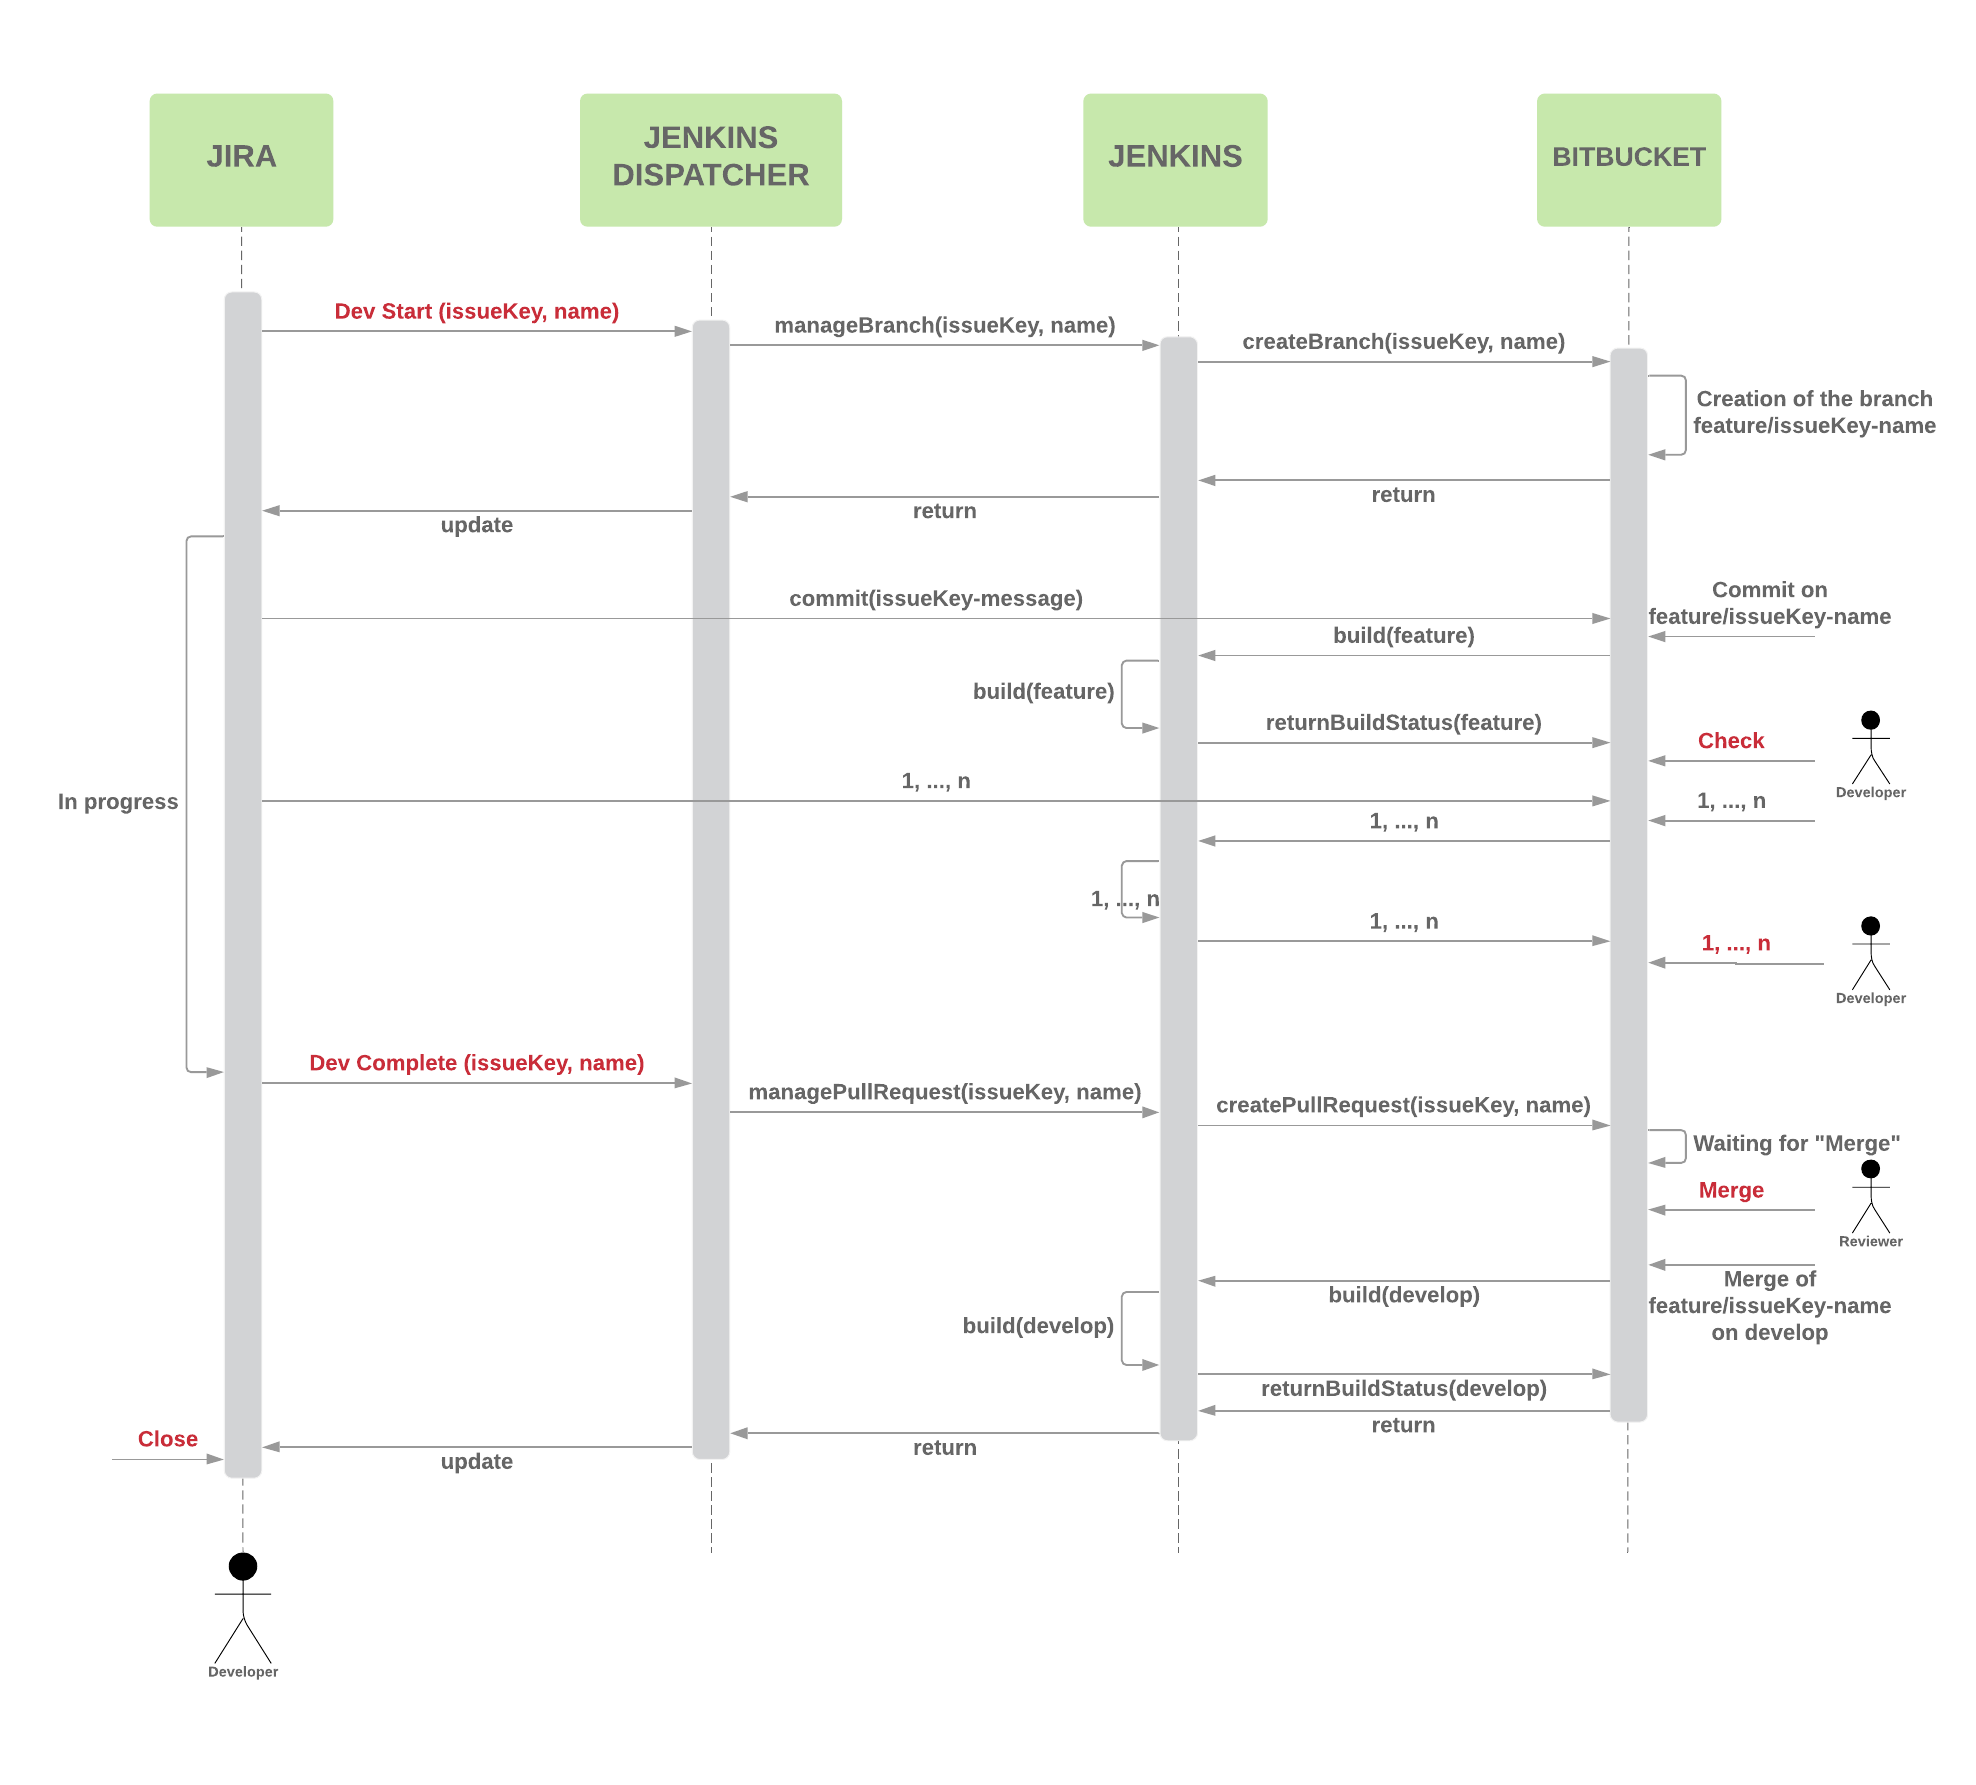
\includegraphics[width=\textwidth]{imgs/devsubtask.png}
    \caption{Diagramma di sequenza di un DevSubtask}
    \label{fig:devSub}
\end{figure}
In riferimento alla figura \ref{fig:devSub} la colonna Jenkins dispatcher rappresenta l'istanza del software incaricata di selezionare lo slave Jenkins (colonna successiva) che  prenderà in carico l'esecuzione della pipeline sulla base di una label inserita nella pipeline di dispatching. 
\\Gli slave sono delle istanze di Jenkins rilasciate all'interno di contenitori gestiti da Openshift tramite le immagini (vedi \ref{containers}) salvate in un registry privato. In questo modo, ogni volta si abbia la necessità di utilizzare un nuovo strumento, è sufficiente creare una nuova immagine che permetta di utilizzarlo senza dover modificare la pipeline sul dispatcher. Questa flessibilità è possibile grazie al sistema di orchestrazione di contenitori di Openshift che garantisce che un nodo specializzato sia sempre attivo e pronto ad eseguire la pipeline.
\\
L'attore di questo scenario è un membro del team di Sviluppo non appena prende in carico l'esecuzione di un DevSubtask. Le operazioni scritte in rosso sono eseguite manualmente dall'utente, mentre quelle in grigio sono integrate nel processo. \\
L'utente scatena il webhook cliccando su "Dev Start", immediatamente viene eseguita la pipeline di manageBranch sul dispatcher utilizzando come parametri la chiave identificativa del DevSubtask ed il nome della feature da implementare. Il dispatcher sceglie il nodo e lancia l'esecuzione della pipeline branchCreation che si occupa di creare un branch nel formato \emph{feature/key-nome} su Bitbucket, Al termine il controllo ritorna al dispatcher che provvede ad aggiornare lo stato del workflow su Jira a "In Progress".\\
Durante lo sviluppo l'utente è incentivato ad effettuare il più frequentemente possibile il push del codice sul proprio branch, infatti, secondo l'approccio della Continuous Integration, quest'azione scatena l'esecuzione del processo di build che permette di rilevare subito se è presente un errore e permette di intervenire immediatamente per correggerlo. Tuttavia per garantire il riferimento a quella determinata feature, è necessario che il messaggio allegato al commit contenga all'inizio della stringa il codice identificativo della issue. Al termine dello sviluppo, l'utente avvia il trigger "Dev Complete" che porta alla creazione di una pull request sul ramo di develop, tale richiesta deve essere revisionata manualmente da un altro membro del team di sviluppo, che, utilizzando il pulsante "Merge" nella sezione dedicata su Bitbucket (in figura \ref{fig:bitbucket-merge}), può decidere se approvare o meno le modifiche effettuate.
\begin{figure}
    \centering
    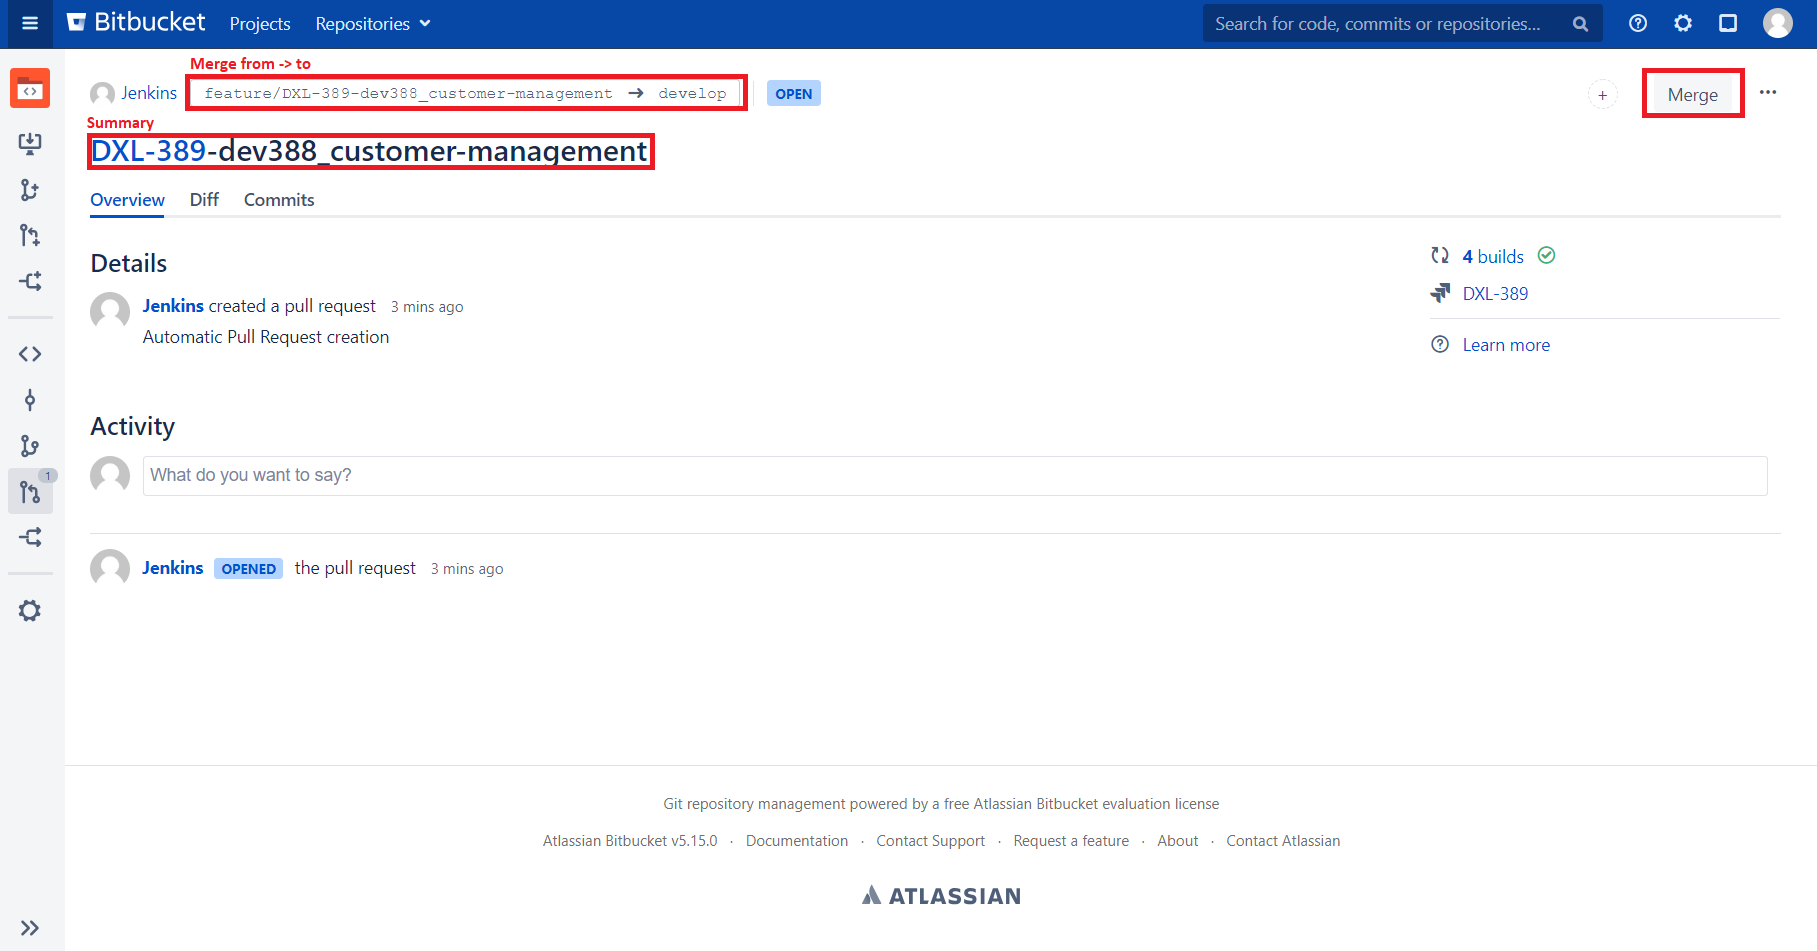
\includegraphics[width=0.9\textwidth]{imgs/bitbucket.png}
    \caption{Interfaccia per la gestione della pull request su Bitbucket.}
    \label{fig:bitbucket-merge}
\end{figure}
All'approvazione tramite il click del pulsante "Merge", viene restituito il comando alla pipeline che provvede ad eseguire la build dell'intero branch di develop (secondo il principio di mantenere sempre il codice stabile e pronto per essere rilasciato) aggiornando numero di build e versione e caricando l'artefatto su un repository. A seconda dell'esito dell'operazione, Jenkins termina l'esecuzione aggiornando lo status del DevSubtask a "Ready to Test". Quando l'utente ha verificato il funzionamento della modifica nell'ambiente di DEV tramite l'issue di Test, il DevSubtask conclude il workflow raggiungendo lo stato di "Done" e lo sviluppatore può considerarlo terminato cliccando sul tasto "Close".

\section{Release Note}
Il processo di notifica dei team prevede l'invio di una mail con allegata una Release Note, ovvero un documento che elenca a livello funzionale le modifiche che sono state rilasciate all'interno della nuova versione del codice.\\
Per la Release Note (da qui in poi abbraviata con RN) integrata all'interno del processo DevOps è necessario soddisfare i seguenti requisiti:
\begin{itemize}
    \item La RN deve contenere l'elenco di tutte le Story rilasciate, assieme ad il nome ed il branch contenente il codice rilasciato in produzione dei componenti coinvolti e, nel caso dell'applicazione a microservizi, uno snapshot contenente la versione attuale di tutti gli oggetti Openshift coinvolti nel rilascio.
    \item La RN deve essere pubblicata su Confluence in uno space dedicato al progetto. Se lo space non è presente deve essere creato in automatico.
    \item La RN deve essere creata nel momento in cui la Release viene rilasciata nell'ambiente di UAT.
    \item La RN deve essere allegata come link ad una mail inviata in automatico al termine della preparazione del documento.
\end{itemize}
La raccolta delle informazioni necessarie per popolare la release note comporta l'utilizzo delle REST API tramite cui invocare la richiesta dei valori con cui popolare la RN. All'interno dell'oggetto Release di Jira sono elencate le Story da rilasciare assieme ai DeploySubtask che contengono i riferimenti ai componenti coinvolti.\\
Per effettuare lo snapshot dello stato dei progetti al momento del rilascio, ho utilizzato un plugin di Jenkins che consente di accedere con comandi semplici alla Openshift Container Platform, in questo modo ho recuperato dai file YAML delle immagini (a cui ho un riferimento grazie al nome del componente) il nome del progetto Openshift in cui sono rilasciate, salvando i valori in una lista che utilizzo successivamente per iterare su tutti i progetti ottenendo una mappa che associa ad ogni progetto la lista dei componenti rilasciati al suo interno.\\
La struttura di una RN deve essere identica a prescindere dalle modifiche effettuate, perciò è stato necessario definire un template HTML rappresentante la pagina di Confluence che viene creata tramite la REST API. Una volta che la struttura è definita nelle sue parti, è necessario popolare dinamicamente i campi di tabelle e variabili, questo è possibile utilizzando un software che permetta il pattern  MVC (vedi \ref{velocity}) come Apache Velocity: inserendo del codice con una particolare sintassi, è possibile definire delle logiche per l'elaborazione delle variabili iniettate nel template, permettendo così la creazione di nuovo codice HTML a seconda del tipo e del numero di variabili passate al contesto, come nell'esempio seguente:
\begin{verbatim}
    <td colspan="1" class="confluenceTd">
        #foreach ($!component in $!components)
           <p><span>#emptyIfNull($!component)</span></p>
        #end
    </td>
\end{verbatim}
La RN è strutturata in modo da avere diverse tabelle, per ogni componente nella lista \emph{components} viene aggiunta una riga alla tabella d'interesse facendo un check sull'elemento e, nel caso esso sia null, restituisce una casella vuota.\\
La pipeline eseguita da Jenkins per la scrittura e l'invio tramite la REST API a Confluence, viene eseguita all'interno del workflow di Release, quando viene eseguito il rilascio nell'ambiente di UAT. \\
\begin{figure}
    \centering
    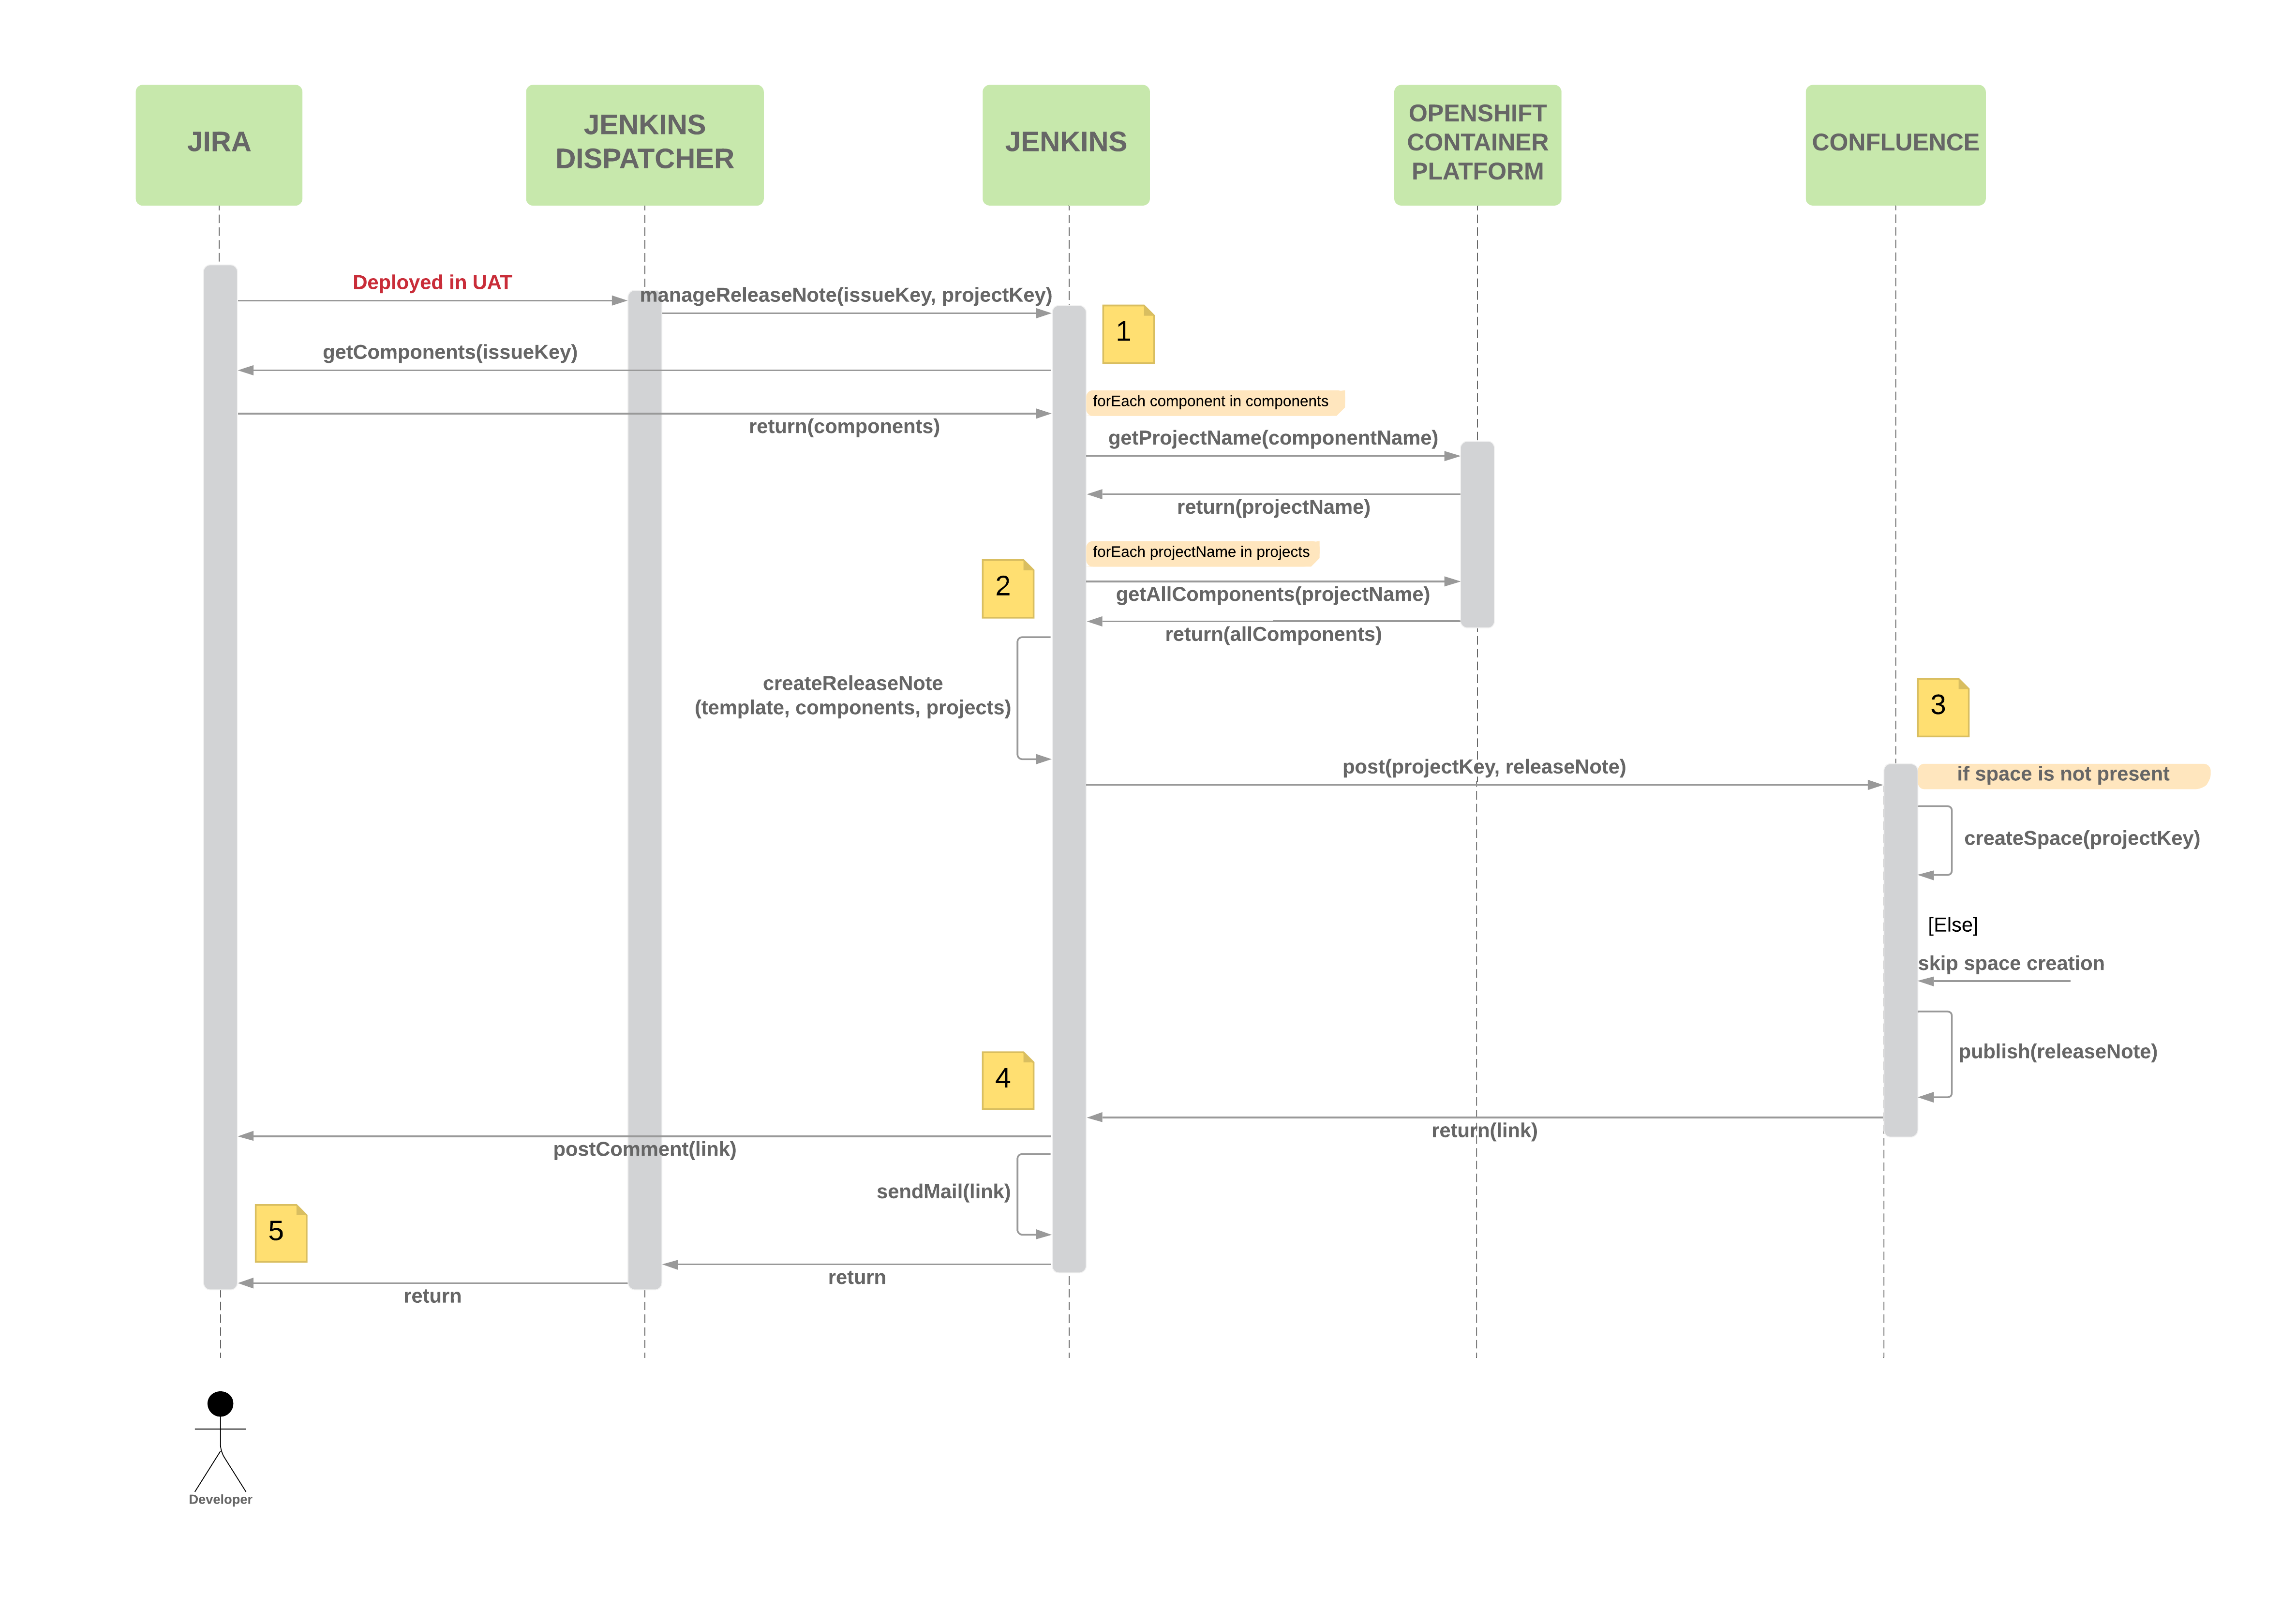
\includegraphics[width=\textwidth]{imgs/ReleaseNoteFlow.png}
    \caption{Flusso descrittivo della pubblicazione della RN su Confluence}
    \label{fig:relNote}
\end{figure}
Il flusso di riferimento è descritto in \ref{fig:relNote}, il trigger è scatenato nel momento in cui l'oggetto Release entra nello stato "Deployed in UAT". Come per la pipeline relativa al subtask di sviluppo, anche in questo caso viene invocato il Jenkins dispatcher che però ora può scegliere un nodo non specializzato perché l'operazione non richiede l'utilizzo di strumenti ad hoc. Il nodo slave scelto dal dispatcher invia una richiesta tramite le REST API per ottenere tutti i componenti che sono inclusi all'interno dell'oggetto Release (passato come parametro al dispatcher) e li salva all'interno di strutture dati per poter essere riutilizzati successivamente (1), stessa cosa avviene per i progetti in cui sono contenuti tali componenti, recuperati tramite il plugin per l'Openshift Container Platform, offerto da Jenkins (2). A questo punto la pipeline ha a disposizione tutte le informazioni necessarie per compilare la RN. Viene inizializzata l'istanza del Velocity Engine e viene scaricato il template HTML da popolare da un repository di Bitbucket. Le strutture dati vengono manipolate in maniera tale da rendere più semplice la visualizzazione nella RN e vengono passate al contesto dato dal template. \\
Una volta che il codice HTML della pagina è pronto per essere pubblicato, tramite una REST API viene invocata la creazione di uno space su Confluence utilizzando la key del progetto come nome, se tale space è già presente (ovvero è già stata pubblicata una RN in precedenza) lo step viene saltato pubblicando direttamente la RN con il titolo projectKey-fixVersion (3). Ultimata la pubblicazione, il link della pagina viene restituito allo slave che lo utilizza per confezionare un commento che viene pubblicato nella pagina riepilogativa della Release su Jira e una mail da inviare ai membri del team di UAT, recuperati da Jira (4). Infine il flusso termina restituendo il controllo al dispatcher che considera terminato il processo (5).\\
Grazie a questo automatismo, lo scambio di informazioni risulta più immediato, più robusto e concentrato in un unico strumento, dove qualunque interessato può visionare ciò che serve, riducendo la probabilità che ci possano essere mancanze od errori. In \ref{fig:release-note} si può vedere un esempio di RN.
\begin{figure}
    \centering
    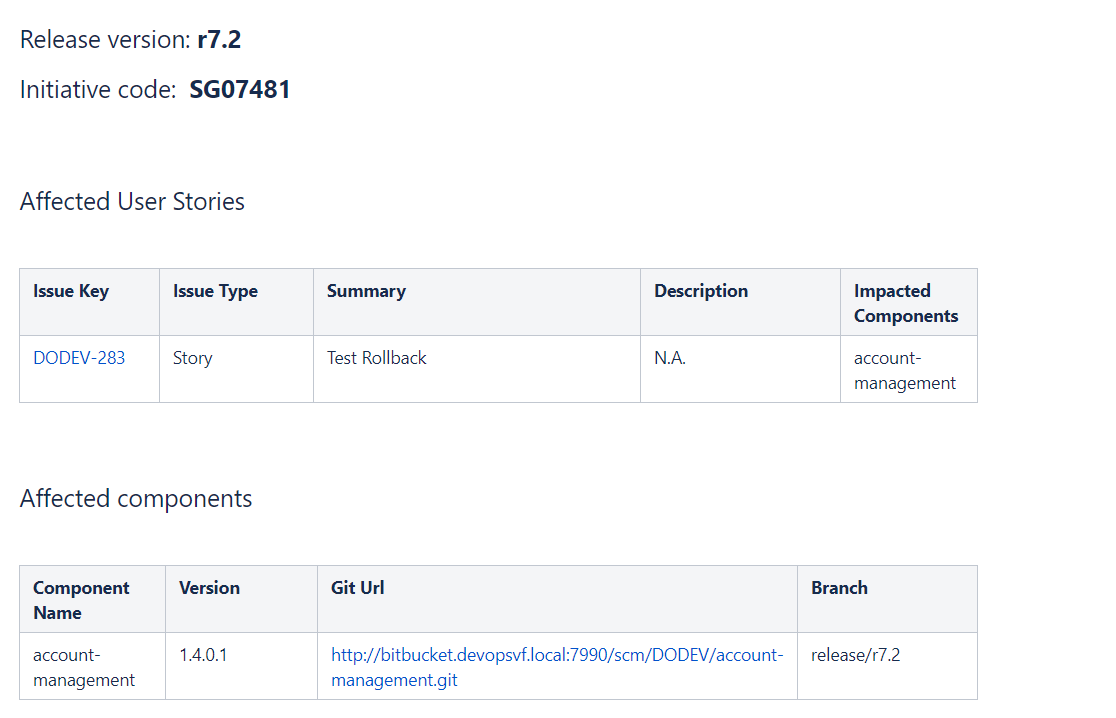
\includegraphics[width=0.9\textwidth]{imgs/release-note.png}
    \caption{Esempio di Release Note.}
    \label{fig:release-note}
\end{figure}

\chapter{Caso d'uso}\label{piattaforma-devops}
In questo capitolo è mostrato un esempio di utilizzo della piattaforma da parte di un'applicazione a microservizi, simulando le diverse richieste di business e tecniche previste nei requisiti.
\section{Implementazione Story o correzione Bug}
Quanto esposto in questo paragrafo descrive il processo relativo ad una user story, ma è applicabile anche alla risoluzione di un bug.\\
Si suppone che il business abbia deciso di introdurre una nuova feature per soddisfare una necessità dovuta all’introduzione di una nuova tecnologia sul mercato.\\
Per sviluppare nuove funzionalità si utilizza il workflow Funzionale, che prevede (ad alto livello):
\begin{enumerate}
    \item Raccolta dei requisiti
    \item Sviluppo
    \item Rilascio in ambiente di DEV e successiva validazione da parte del team di sviluppo
    \item Promozione nell’ambiente di TEST e successiva validazione nel caso non vi siano fallimenti sui test
    \item Promozione nell’ambiente di UAT e successiva validazione nel caso non vi siano fallimenti sui test
    \item Rilascio in PROD
\end{enumerate}
Il business descrive ad alto livello la nuova funzionalità che deve essere acquisita dall’applicazione e la carica su Confluence, dopodiché il team funzionale si occupa di trasformarla nella forma di User Story creando un task di tipologia Story (che segue il workflow funzionale) su Jira (\ref{fig:jira-story}).
\begin{figure}
    \centering
    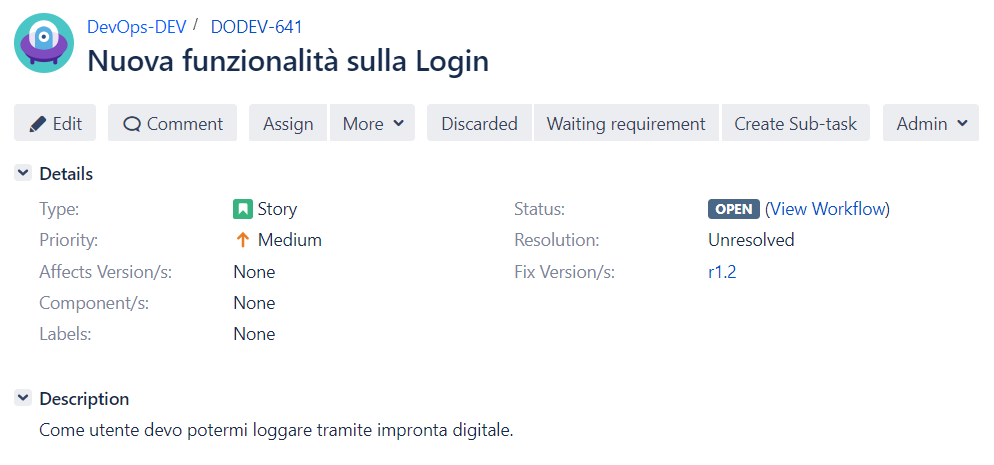
\includegraphics[width=0.9\textwidth]{imgs/story.png}
    \caption{Pagina riepilogativa di una Story}
    \label{fig:jira-story}
\end{figure}
Una volta che la Story viene definita rimane immutabile e il team di sviluppo può prenderla in carico per implementare la funzionalità sul codice. È importante evidenziare nella figura \ref{fig:jira-story} il campo Fix Version: il valore presente indica la release in cui quella funzionalità viene rilasciata.\\
Un issue di tipologia Story può essere formata da una serie di task a grana più fine, chiamati DevSubtask che comprendono le singole modifiche necessarie ai vari componenti (e.g. microservizi, classi o metodi), per poter implementare la funzionalità.\\
Un issue DevSubtask segue il workflow omonimo, così composto:
\begin{enumerate}
    \item To Do
    \item In progress
    \item Ready to merge
    \item Ready to deploy
    \item Ready to test
    \item Done
\end{enumerate}
Una volta che uno o più DevSubtask vengono creati, un membro del team di sviluppo può prendere in carico uno o più subtask e iniziare lo sviluppo. Egli scatena manualmente il trigger “DEV START” nell’oggetto DevSubtask ed automaticamente: la Story passa nello stato “IN PROGRESS”; viene creato un branch di feature per la modifica a partire dal ramo di develop, se si tratta di una Story o Bug, o master, se si tratta di un Hotfix (secondo il modello Git workflow). Lo sviluppatore clona il repository ed effettua il checkout del branch appena creato, effettua le modifiche che ritiene necessarie. Quando ritiene che il lavoro di sviluppo sia terminato, effettua il push del proprio repository e preme il pulsante di “DEV COMPLETE” che scatena la creazione di una pull request\footnote{Una richiesta di merge della propria feature sul branch develop, in questo modo il codice deve passare per l’approvazione di un altro membro del team.} sul repository che deve essere approvata manualmente da un membro del team di sviluppo. Quando la pull request viene accettata, Jenkins scatena automaticamente la build del codice (che comprende: test unitari, analisi statica, analisi di qualità del codice, la creazione dell’immagine – nel caso di microservizi) e, successivamente, l’aggiornamento dello stato del DevSubtask in “READY TO DEPLOY”. Quando il DevSubtask viene rilasciato in DEV, il suo stato passa a “READY TO TEST” (vedere paragrafo successivo), se anche i Test vanno a buon fine, lo sviluppatore può dichiarare il DevSubtask come “DONE”.\\
Quando tutti i DevSubtask di una Story vengono dichiarati DONE, essa passa nello stato di “VALIDATED ON DEV, una Story rimane in questo stato fino a quando non viene inclusa in una Release.


\section{Test della funzionalità}
La funzionalità è stata sviluppata,a ma bisogna verificare che soddisfi tutti i requisiti e che che venga testata per individuare il prima possibile eventuali bug o regressioni.\\
Una volta che una User Story risulta completata e rilasciata su DEV, per poter essere validata deve superare un insieme di test, unitari o meno. I test sono concordati e scritti sia dagli sviluppatori che dai membri del team di QA, e sono raggruppati all’interno dell’oggetto test, vengono eseguiti su ogni issue a cui sono collegati. I report con i risultati dei test sono prodotti in diversi formati a seconda della tipologia (JSON, XML, HTML), attraverso l’utilizzo di una piccola applicazione Java vengono elaborati per poter essere integrati nel report presente sulla pagina dell’issue di test.\\
\begin{figure}
    \centering
    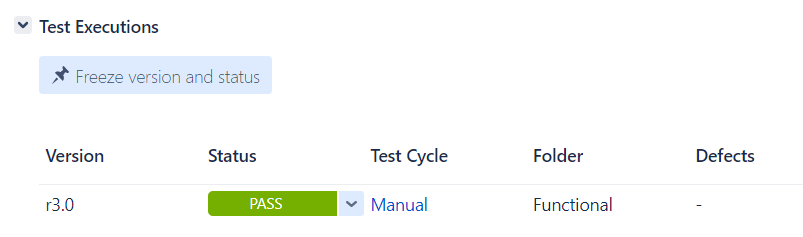
\includegraphics[width=0.9\textwidth]{imgs/test-ok.png}
    \caption{Esecuzione positiva di un Test}
    \label{fig:test-ko}
\end{figure}
Nel caso un test fallisca viene automaticamente creata un issue di tipo Bug (figura \ref{fig:bug}) mantenendo le informazioni relative al Test che è andato in fallimento (figura \ref{fig:test-ko}).l\\
\begin{figure}
    \centering
    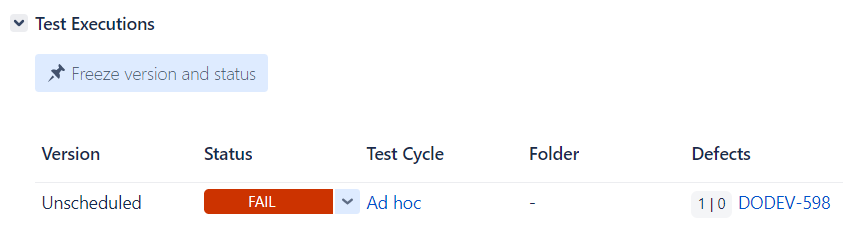
\includegraphics[width=0.9\textwidth]{imgs/test-ko.png}
    \caption{Esecuzione negativa di un Test}
    \label{fig:test-ok}
\end{figure}
\begin{figure}
    \centering
    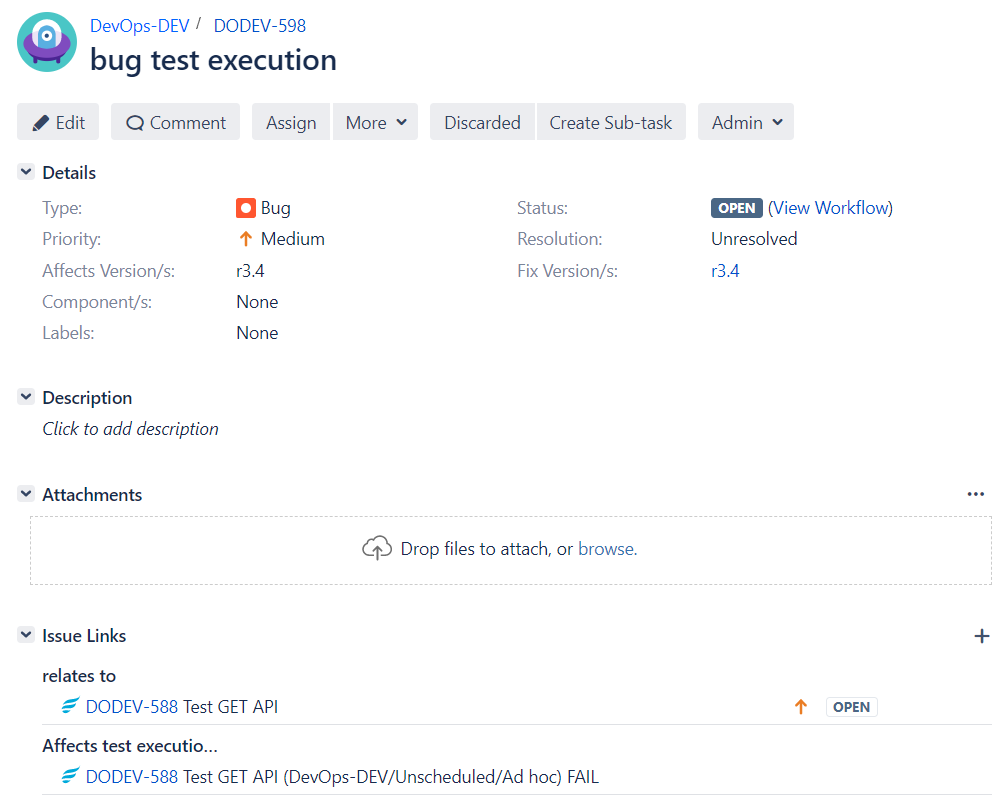
\includegraphics[width=0.9\textwidth]{imgs/bug.png}
    \caption{Bug automaticamente creato al fallimento del Test}
    \label{fig:bug}
\end{figure}
Nel caso in cui i Test diano tutti esito positivo (figura \ref{fig:test-ok}), la funzionalità può essere validata su DEV ed è pronta per la promozione in TEST.
\section{Correzione di un bug critico in produzione - Hotfix}
Il team di Operations riceve la segnalazione di un bug in produzione che non permette all’utente di sottomettere un ordine all’interno dello shop dell’applicazione. È una criticità ad alto impatto per il business in quanto inibisce un canale di vendita dell’azienda, di conseguenza è necessario un intervento immediato.\\
Il team funzionale crea una issue di tipo Hotfix, con tutte le informazioni necessarie al team di sviluppo per individuare l’errore e fixarlo. Il procedimento di risoluzione lato sviluppo è identico a quello per l’implementazione di una Story o di un Bug, ovvero vengono creati dei DevSubtask (in questo caso creeranno un branch a partire dal ramo master) vengono presi in carico, completati e testati tramite l’issue di tipo Test, la differenza è nel ramo di partenza, non "develop", ma "master".\\ Quando l’Hotfix è pronto per andare in produzione, viene creato un oggetto Release con un campo “type” aggiornato con il valore “hotfix” per distinguerla da una regolare Release. 
\begin{figure}
    \centering
    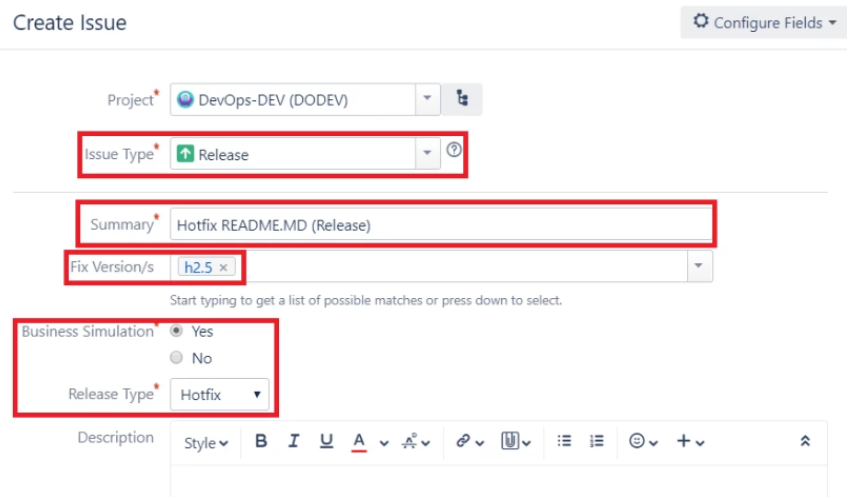
\includegraphics[width=0.9\textwidth]{imgs/hotfix.PNG}
    \caption{Esempio di una Release per un Hotfix.}
    \label{fig:hotfix-release}
\end{figure}

\section{Procedura di Release}
Quando i requisiti dello sprint sono stati sviluppati e testati, devono essere rilasciati in produzione. \\
Quando le Story che devono essere rilasciate sono nello stato “VALIDATED ON DEV”, il team di sviluppo crea un oggetto di tipo Release con la stessa fix version delle Story che devono essere rilasciate che verranno automaticamente incluse.\\
L’issue di tipo Release segue l’omonimo workflow:
\begin{enumerate}
    \item Package preparation
    \item Ready to Release
    \item Released on TEST
    \item Validated on TEST
    \item Package preparation
    \item Ready to Release
    \item Released on UAT
    \item Validated on UAT
    \item Package preparation
    \item Ready to Release
    \item Released on PROD
\end{enumerate}
Il valore per l’ambiente di rilascio è inizialmente settato con la stringa TEST, perché quando l’oggetto Release viene creato, tutte le Story e i Bug si trovano nello stato “VALIDATED ON DEV” e quindi pronte per essere rilasciate nell’ambiente di TEST.
A seconda delle Story che sono comprese nella Release, automaticamente vengono creati dei DeploySubtask (uno per ogni DevSubtask di ogni Story, se ho due Story con tre DevSubtask ciascuno, avrò sei DeploySubtask), ognuno di essi segue il workflow omonimo che prevede:
\begin{enumerate}
    \item Package preparation
    \item Ready to Deploy
    \item Deployed
    \item Done
\end{enumerate}
\begin{figure}[H]
    \centering
    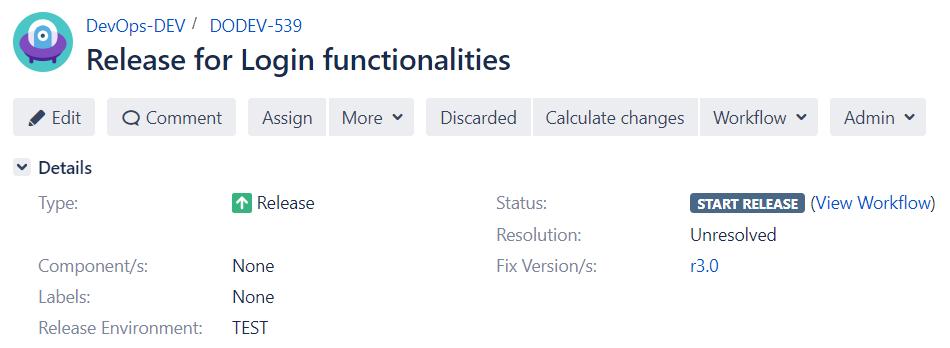
\includegraphics[width=0.9\textwidth]{imgs/release.png}
    \caption{Esempio di una issue di tipo Release.}
    \label{fig:release}
\end{figure}
Quando viene eseguito il trigger di “Prepare Package” sia la Release che i DeploySubtask entrano nello stato di “PACKAGE PREPARATION” e automaticamente viene creato un branch nella forma “release/fix-version-number” a partire dal branch develop. Una volta terminata la preparazione e che tutti i DeploySubtask entrano nello stato “READY TO DEPLOY”, lo stato della Release viene aggiornato a “READY TO RELEASE”.\\
A questo punto è possibile eseguire il rilascio nell’ambiente di TEST tramite l’esecuzione del comando “Release”, una volta terminato il processo, la Release passa nello stato “RELEASED ON TEST” e le Story collegate passano nello stato “DEPLOYED ON TEST”.\\
Per poter passare all’ambiente successivo, le Story devono essere validate nell’ambiente di TEST dal team di sviluppo. Quando tutte le Story sono nello stato “VALIDATED ON TEST”, la Release passa in “APPROVAL FOR UAT”.\\
In questo punto del processo viene inviata una notifica al team di UAT con un link ad una Release Note\footnote{Documento che elenca le modifiche introdotte sul software nella release in oggetto.}, creata in automatico tramite un template HTML popolato con Velocity e pubblicato su Confluence in uno space dedicato per il progetto, dove sono elencate le informazioni necessarie per prendere rapidamente visione di ciò che è stato implementato (vedi figura \ref{fig:release-note}).\\
Un membro del team di UAT può cliccare sul trigger “Release ready” facendo aggiornare in automatico il campo “Release environment” con il valore “UAT”. Quindi si può eseguire il trigger di “Release” che scatena gli stessi passaggi visti nel rilascio nell’ambiente di TEST.\\
Terminato il processo di rilascio, il team di UAT può eseguire i test End-to-End e verificare che tutto si comporti secondo attese e lo stato della Release viene aggiornato a “RELEASED ON UAT”, i DeploySubtask risultano “DEPLOYED” e le Story “VALIDATED ON UAT”.\\
Per abilitare lo step successivo, una volta terminati i test, il team di UAT clicca sul trigger “APPROVAL FOR PROD”, dopodiché il processo provvede ad inviare una notifica con allegata la Release Note al team di Operations, che provvede a loggarsi e a cliccare su “RELEASE READY” per aggiornare il campo di “release environment” al valore di “PROD” e gli stati dei DeploySubtask e delle Story. Infine il team clicca sul comando “Go Live” per lanciare la procedura di rilascio nell’ambiente di produzione.\\
Se la procedura va a buon fine, ad ogni DeploySubtask vengono aggiunti dei campi per evidenziare la versione corrente rilasciata e la versione precedente (utile in caso di rollback).
\begin{figure}
    \centering
    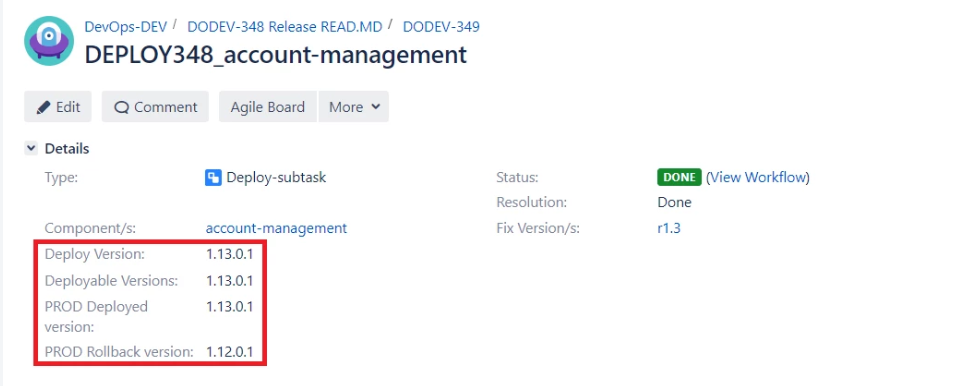
\includegraphics[width=0.9\textwidth]{imgs/deploy-subtask.png}
    \caption{Aggiornamento dei campi nel DeploySubtask.}
    \label{fig:deploy-subtask}
\end{figure}
A questo punto del processo, le funzionalità sono online e disponibili agli utenti. In caso di malfunzionamenti critici è sempre possibile effettuare una procedura di rollback effettuando una Release della versione precedente dei DeploySubtask.


%\chapter{Risultati raggiunti}

% CONCLUSIONI
\chapter*{Conclusioni}\label{conclusioni}
\addcontentsline{toc}{chapter}{Conclusioni}


% ELENCO DELLE FIGURE (OPZIONALE)
\addcontentsline{toc}{chapter}{Elenco delle figure}
\listoffigures


% BIBLIOGRAFIA
\addcontentsline{toc}{chapter}{Bibliografia}
\begin{thebibliography}{9}
        \bibitem{manifesto-agile}
            \emph{''Manifesto per lo sviluppo agile del software''},
        http://agilemanifesto.org
        
        \bibitem{palmquist-agile}PALMQUIST, M. Steven, et al.
            \emph{``Parallel worlds: Agile and waterfall differences and similarities''},
          CARNEGIE-MELLON UNIV PITTSBURGH PA SOFTWARE ENGINEERING INST, 2013, p. 4-5
          
          \bibitem{balaji-agile}BALAJI, S.; MURUGAIYAN, M. Sundararajan.
            \emph{''Waterfall vs. V-Model vs. Agile: A comparative study on SDLC''},
            International Journal of Information Technology and Business Management, 2012, 2.1: 26-30
            
        \bibitem{kumar-agile}KUMAR, Gaurav; BHATIA, Pradeep Kumar.
            \emph{''Impact of agile methodology on software development process''},
            International Journal of Computer Technology and Electronics Engineering (IJCTEE), 2012, 2.4: 46-50
            
        \bibitem{melo-agile}MELO, Claudia De O., et al.
            \emph{''Interpretative case studies on agile team productivity and management''},
            Information and Software Technology, 2013, 55.2: 412-427
            
        \bibitem{kniberg-agile}KNIBERG, Henrik.
            \emph{''Kanban vs Scrum''},
            Crisp AB. Viitattu, 2009, 1: 1-41
            
        \bibitem{schwaber-agile}SCHWABER, Ken.
            \emph{''Scrum development process''},
            Business object design and implementation. Springer, London, 1997, p. 117-134
            
        \bibitem{klipp-agile}KLIPP, Paul.
            \emph{''Getting started with Kanban''},
            Kanbanery, 2011
            
        \bibitem{hasnain-agile}HASNAIN, Eisha; HALL, Tracy.
            \emph{''Introduction to Stand Up Meetings in Agile Methods''},
            AIP Conference Proceedings. AIP, 2009. p. 110-120
            
        \bibitem{garfinkel-agile}GARFINKEL, Simson.
            \emph{''History’s worst software bugs''},
            Wired News, Nov, 2005
            
        \bibitem{wikipedia-devops-agile}
            \emph{''DevOps: la metodologia che unisce IT e Business''},
            https://tuttiperlinux.blog, 2015.
            
        \bibitem{chen-devops}CHEN, Lianping.
            \emph{''Continuous delivery: Huge benefits, but challenges too''},
            IEEE Software, 2015, 32.2: 50-54
            
        \bibitem{balalaie-devops}BALALAIE, Armin; HEYDARNOORI, Abbas; JAMSHIDI, Pooyan.
            \emph{''Microservices architecture enables devops: Migration to a cloud-native architecture''},
            IEEE Software, 2016, 33.3: 42-52
            
        \bibitem{lwakatare-devops}LWAKATARE, Lucy Ellen; KUVAJA, Pasi; OIVO, Markku.
            \emph{''Relationship of DevOps to Agile, Lean and Continuous Deployment''},
            International Conference on Product-Focused Software Process Improvement. Springer, Cham, 2016. p. 399-415
            
        \bibitem{balalaie-devops}BALALAIE, Armin; HEYDARNOORI, Abbas; JAMSHIDI, Pooyan.
            \emph{''Microservices architecture enables devops: Migration to a cloud-native architecture''},
            IEEE Software, 2016, 33.3: 42-52
        
        \bibitem{humble-devops}HUMBLE, Jez; FARLEY, David.
            \emph{''Continuous Delivery: reliable software releases through build, test, and deployment automation''},
            Pearson Education Inc. ISBN 978-0-321-60191-9, 2011
            
        \bibitem{fowler-ci}FOWLER, Martin.
            \emph{''Continuous Integration''},
            https://martinfowler.com, 2006
        
        \bibitem{hutterman-iac}HÜTTERMANN, Michael. 
            \emph{''DevOps for Developers.''},
            Apress, Berkeley, CA, 2012. p. 135-156
            
        \bibitem{clark-automation}CLARK, Mike.
            \emph{''Pragmatic project automation: how to build, deploy, and monitor Java applications''},
            The Pragmatic Programmers, LLC, 2004
            
        \bibitem{driessen-gitflow}DRIESSEN, Vincent.
            \emph{''A successful Git branching model''},
            https://nvie.com, 2010
            
        \bibitem{atlassian-doc}
            \emph{''Gitflow workflow''},
            https://it.atlassian.com  
            
        \bibitem{felter-containers}FELTER, Wes, et al.
            \emph{''An updated performance comparison of virtual machines and linux containers''},
            IEEE international symposium on performance analysis of systems and software (ISPASS). IEEE, 2015. p. 171-172
            
        \bibitem{strachan-kubernetes}STRACHAN, James.
            \emph{''Kubernetes for developers''},
            https://blog.fabric8.io, 2015
            
        \bibitem{cabibbo}CABIBBO, Luca.
            \emph{''Orchestrazione di contenitori''},
            http://cabibbo.dia.uniroma3.it, 2018
            
        \bibitem{scrum-ruoli}
            \emph{''I ruoli in Scrum''},
            https://www.imlearning.it
            
        \bibitem{gruver-agile}GRUVER, Gary; MOUSER, Tommy.
            \emph{''Leading the transformation: Applying agile and devops principles at scale''},
            IT Revolution, 2015
            
        \bibitem{myrbakken-devsecops}MYRBAKKEN, Håvard; COLOMO-PALACIOS, Ricardo
            \emph{''DevSecOps: a multivocal literature review''},
            International Conference on Software Process Improvement and Capability Determination. Springer, Cham, 2017. p. 17-29
            
        \bibitem{opensource-vs-proprietary}
            \emph{''Open Source vs Proprietary Software Pros and Cons''},
            http://www.optimusinfo.com
            
        \bibitem{opensource-vs-proprietary-bugs}ASAY, Matt.
            \emph{''Open-source vs. proprietary software bugs: Which get squashed fastest?''},
            https://www.cnet.com, 2007
            
        \bibitem{bugzilla-doc}
            \emph{''Lifecycle of a Bug''},
            https://bugzilla.readthedocs.io
            
        \bibitem{svn-docs}
            \emph{''Subversion's architecture''},
            http://svnbook.red-bean.com
            
        \bibitem{git-docs}
            \emph{''Git's architecture''},
            https://www.edureka.co
            
        \bibitem{ci-env}SYED, Shahbaz Ali; TARIQ, Rahim Soomro.
            \emph{''Achieving Software Release Management and Continuous Integration using Maven, Jenkins and Artifactory''},
            International Journal of Experiential Learning & Case Studies 3.2 (2018): 236-245.
            
        \bibitem{jenkins-docs}
            \emph{''Syntax Comparison''},
            https://jenkins.io
            
            
        %\bibitem{build-tools}
        %    \emph{''Build tools''},
        %    https://technologyconversations.com, 2014
            
        \bibitem{kubernetes-vs-openshift}CHOLEWA, Tomasz.
            \emph{''10 most important differences between OpenShift and Kubernetes''},
            https://cloudowski.com, 2018
        
        %\bibitem{}
        %    \emph{''''},
        %
        %\bibitem{}
        %    \emph{''''},
        %
        %\bibitem{}
        %    \emph{''''},
        %
        %\bibitem{}
        %    \emph{''''},
            
            
\end{thebibliography}


\end{document}
